% The ranking reads generated receipt macros. Supplemental tables read the bound aggregate CSVs.
% The paper checker rejects typed digits in prose and the PDF build verifies supplemental inputs.
\documentclass[10pt,letterpaper]{article}
\pdfminorversion=7
\usepackage[T1]{fontenc}
\usepackage[utf8]{inputenc}
\usepackage{charter}
\usepackage[scaled=0.92]{helvet}
\usepackage{lmodern}
\renewcommand{\rmdefault}{bch}
\usepackage[letterpaper,textwidth=6.7in,textheight=9in,centering]{geometry}
\usepackage{amsmath,amssymb}
\usepackage{booktabs,tabularx}
\usepackage{makecell}
\usepackage{graphicx}
\usepackage{pgfplots,pgfplotstable}
\pgfplotsset{compat=1.18}
\usetikzlibrary{arrows.meta,positioning}
\usepackage{xcolor}
\usepackage{titlesec}
\usepackage{natbib}
\usepackage{microtype}
\usepackage{enumitem}
\usepackage[font=small,labelfont=bf]{caption}
\usepackage{url}
\usepackage[colorlinks=true,linkcolor=blue!50!black,citecolor=blue!50!black,urlcolor=blue!50!black]{hyperref}

% Generated by docs/whitepaper-v3/scripts/render_v3_paper.py -- DO NOT EDIT BY HAND.
\newcommand{\VThree}[1]{\ifcsname VThree@#1\endcsname\csname VThree@#1\endcsname\else\PackageError{dope-v3}{undefined receipt macro #1}{Re-run render_v3_paper.py}\fi}
\expandafter\newcommand\csname VThree@ReleaseVersion\endcsname{v3.0.0}
\expandafter\newcommand\csname VThree@BaseVersion\endcsname{2.0.0}
\expandafter\newcommand\csname VThree@OldVersion\endcsname{1.3.0}
\expandafter\newcommand\csname VThree@PrimarySha\endcsname{55974867a938}
\expandafter\newcommand\csname VThree@CompareSha\endcsname{5ac5a9bd0d49}
\expandafter\newcommand\csname VThree@KpiContractSha\endcsname{200ea0ed1ba2}
\expandafter\newcommand\csname VThree@EvLayoutSha\endcsname{e99647eb75cd}
\expandafter\newcommand\csname VThree@ScheduleSha\endcsname{14238f1d5b9e}
\expandafter\newcommand\csname VThree@ToolVersion\endcsname{2.0.0}
\expandafter\newcommand\csname VThree@ToolGitSha\endcsname{unset}
\expandafter\newcommand\csname VThree@ProtocolFrozen\endcsname{false}
\expandafter\newcommand\csname VThree@BootDraws\endcsname{10{,}000}
\expandafter\newcommand\csname VThree@Scheduled\endcsname{64}
\expandafter\newcommand\csname VThree@Uninformative\endcsname{20}
\expandafter\newcommand\csname VThree@Families\endcsname{11}
\expandafter\newcommand\csname VThree@ArmCount\endcsname{11}
\expandafter\newcommand\csname VThree@ThirdPartyCount\endcsname{0}
\expandafter\newcommand\csname VThree@DseHeaderBytes\endcsname{24}
\expandafter\newcommand\csname VThree@CrcBytes\endcsname{4}
\expandafter\newcommand\csname VThree@TlvBytes\endcsname{3}
\expandafter\newcommand\csname VThree@MargBaseBytes\endcsname{6}
\expandafter\newcommand\csname VThree@LinFixedBytes\endcsname{2}
\expandafter\newcommand\csname VThree@LinPerOutBytes\endcsname{8}
\expandafter\newcommand\csname VThree@EffectBytes\endcsname{12}
\expandafter\newcommand\csname VThree@PairBytes\endcsname{5}
\expandafter\newcommand\csname VThree@TreeBytes\endcsname{14}
\expandafter\newcommand\csname VThree@TreeLeaves\endcsname{8}
\expandafter\newcommand\csname VThree@MaxTrees\endcsname{40}
\expandafter\newcommand\csname VThree@EffectBins\endcsname{8}
\expandafter\newcommand\csname VThree@MaxEffects\endcsname{24}
\expandafter\newcommand\csname VThree@MaxPairs\endcsname{24}
\expandafter\newcommand\csname VThree@MaxCols\endcsname{64}
\expandafter\newcommand\csname VThree@MaxClasses\endcsname{8}
\expandafter\newcommand\csname VThree@MaxRank\endcsname{12}
\expandafter\newcommand\csname VThree@MaxRegimes\endcsname{8}
\expandafter\newcommand\csname VThree@KnotCount\endcsname{17}
\expandafter\newcommand\csname VThree@DpaHeaderBytes\endcsname{13}
\expandafter\newcommand\csname VThree@MinPacketRoom\endcsname{96}
\expandafter\newcommand\csname VThree@CliBudget\endcsname{2{,}048}
\expandafter\newcommand\csname VThree@FoldVeto\endcsname{0.05}
\expandafter\newcommand\csname VThree@MinTestPerClass\endcsname{5}
\expandafter\newcommand\csname VThree@MinCheckGroups\endcsname{80}
\expandafter\newcommand\csname VThree@CheckSynthFactor\endcsname{2}
\expandafter\newcommand\csname VThree@SelectionMargin\endcsname{0.02}
\expandafter\newcommand\csname VThree@TreeDepth\endcsname{3}
\expandafter\newcommand\csname VThree@RegressionFamilies\endcsname{4}
\expandafter\newcommand\csname VThree@BinaryFamilies\endcsname{3}
\expandafter\newcommand\csname VThree@MulticlassFamilies\endcsname{4}
\expandafter\newcommand\csname VThree@ContractId\endcsname{\texttt{dope-kpi/v2}}
\expandafter\newcommand\csname VThree@ContractStatus\endcsname{candidate}
\expandafter\newcommand\csname VThree@ClipLow\endcsname{\ensuremath{-}1}
\expandafter\newcommand\csname VThree@ClipHigh\endcsname{1.25}
\expandafter\newcommand\csname VThree@FailedValue\endcsname{\ensuremath{-}1}
\expandafter\newcommand\csname VThree@PrimaryMult\endcsname{4}
\expandafter\newcommand\csname VThree@CiLevel\endcsname{95\%}
\expandafter\newcommand\csname VThree@LowerPct\endcsname{2.5}
\expandafter\newcommand\csname VThree@UpperPct\endcsname{97.5}
\expandafter\newcommand\csname VThree@HolmAlpha\endcsname{0.05}
\expandafter\newcommand\csname VThree@MinDelta\endcsname{0.01}
\expandafter\newcommand\csname VThree@CiLowGt\endcsname{0}
\expandafter\newcommand\csname VThree@TaskCiLowGt\endcsname{\ensuremath{-}0.02}
\expandafter\newcommand\csname VThree@MlpDeltaGe\endcsname{0}
\expandafter\newcommand\csname VThree@RealismDeltaGt\endcsname{\ensuremath{-}0.03}
\expandafter\newcommand\csname VThree@PrivacyDeltaGt\endcsname{\ensuremath{-}0.03}
\expandafter\newcommand\csname VThree@CopyLe\endcsname{0.005}
\expandafter\newcommand\csname VThree@NullMaxRatePct\endcsname{5\%}
\expandafter\newcommand\csname VThree@BudgetBytes\endcsname{2{,}048}
\expandafter\newcommand\csname VThree@BudgetKiB\endcsname{2}
\expandafter\newcommand\csname VThree@C2stMax\endcsname{0.7}
\expandafter\newcommand\csname VThree@MargAucMax\endcsname{0.6}
\expandafter\newcommand\csname VThree@RuleViolationMax\endcsname{2}
\expandafter\newcommand\csname VThree@DcrMax\endcsname{0.55}
\expandafter\newcommand\csname VThree@MiaAucMax\endcsname{0.55}
\expandafter\newcommand\csname VThree@MiaTprMax\endcsname{0.02}
\expandafter\newcommand\csname VThree@MiaFprPct\endcsname{1\%}
\expandafter\newcommand\csname VThree@SupportK\endcsname{10}
\expandafter\newcommand\csname VThree@EvTiers\endcsname{4}
\expandafter\newcommand\csname VThree@EvColDim\endcsname{128}
\expandafter\newcommand\csname VThree@EvEdgeDim\endcsname{16}
\expandafter\newcommand\csname VThree@EvClassDim\endcsname{16}
\expandafter\newcommand\csname VThree@EvClassColDim\endcsname{4}
\expandafter\newcommand\csname VThree@EvGroupDim\endcsname{8}
\expandafter\newcommand\csname VThree@EvGlobDim\endcsname{160}
\expandafter\newcommand\csname VThree@CandId\endcsname{\texttt{dope-v3b-auto-v8}}
\expandafter\newcommand\csname VThree@CandTrg\endcsname{\ensuremath{-}0.121 [\ensuremath{-}0.189, \ensuremath{-}0.049]}
\expandafter\newcommand\csname VThree@CandTrgPoint\endcsname{\ensuremath{-}0.121}
\expandafter\newcommand\csname VThree@CandMatched\endcsname{\ensuremath{-}0.309 [\ensuremath{-}0.488, \ensuremath{-}0.171]}
\expandafter\newcommand\csname VThree@CandMlp\endcsname{\ensuremath{-}0.349}
\expandafter\newcommand\csname VThree@CandFailed\endcsname{0}
\expandafter\newcommand\csname VThree@CandCells\endcsname{44}
\expandafter\newcommand\csname VThree@CandNotApplicable\endcsname{0}
\expandafter\newcommand\csname VThree@CandC2st\endcsname{0.967}
\expandafter\newcommand\csname VThree@CandRegression\endcsname{\ensuremath{-}0.137}
\expandafter\newcommand\csname VThree@CandBinary\endcsname{\ensuremath{-}0.136}
\expandafter\newcommand\csname VThree@CandMulticlass\endcsname{\ensuremath{-}0.089}
\expandafter\newcommand\csname VThree@CandBytesMed\endcsname{1{,}787}
\expandafter\newcommand\csname VThree@CandBytesMax\endcsname{2{,}048}
\expandafter\newcommand\csname VThree@CandRealism\endcsname{0.194}
\expandafter\newcommand\csname VThree@CandPrivacy\endcsname{0.688}
\expandafter\newcommand\csname VThree@CandRetLinear\endcsname{0.942}
\expandafter\newcommand\csname VThree@CandRetGbdt\endcsname{0.916}
\expandafter\newcommand\csname VThree@CandRetMlp\endcsname{0.792}
\expandafter\newcommand\csname VThree@BaseId\endcsname{\texttt{dope-2.0.0-auto}}
\expandafter\newcommand\csname VThree@BaseTrg\endcsname{\ensuremath{-}0.181 [\ensuremath{-}0.280, \ensuremath{-}0.085]}
\expandafter\newcommand\csname VThree@BaseTrgPoint\endcsname{\ensuremath{-}0.181}
\expandafter\newcommand\csname VThree@BaseMatched\endcsname{\ensuremath{-}0.333 [\ensuremath{-}0.513, \ensuremath{-}0.174]}
\expandafter\newcommand\csname VThree@BaseMlp\endcsname{\ensuremath{-}0.341}
\expandafter\newcommand\csname VThree@BaseFailed\endcsname{0}
\expandafter\newcommand\csname VThree@BaseCells\endcsname{44}
\expandafter\newcommand\csname VThree@BaseNotApplicable\endcsname{0}
\expandafter\newcommand\csname VThree@BaseC2st\endcsname{0.958}
\expandafter\newcommand\csname VThree@BaseRegression\endcsname{\ensuremath{-}0.118}
\expandafter\newcommand\csname VThree@BaseBinary\endcsname{\ensuremath{-}0.278}
\expandafter\newcommand\csname VThree@BaseMulticlass\endcsname{\ensuremath{-}0.146}
\expandafter\newcommand\csname VThree@BaseBytesMed\endcsname{1{,}817.5}
\expandafter\newcommand\csname VThree@BaseBytesMax\endcsname{2{,}048}
\expandafter\newcommand\csname VThree@BaseRealism\endcsname{0.306}
\expandafter\newcommand\csname VThree@BasePrivacy\endcsname{0.719}
\expandafter\newcommand\csname VThree@BaseRetLinear\endcsname{0.939}
\expandafter\newcommand\csname VThree@BaseRetGbdt\endcsname{0.917}
\expandafter\newcommand\csname VThree@BaseRetMlp\endcsname{0.792}
\expandafter\newcommand\csname VThree@AnalyticId\endcsname{\texttt{dse8-p0-v3b}}
\expandafter\newcommand\csname VThree@AnalyticTrg\endcsname{\ensuremath{-}0.342 [\ensuremath{-}0.652, \ensuremath{-}0.103]}
\expandafter\newcommand\csname VThree@AnalyticTrgPoint\endcsname{\ensuremath{-}0.342}
\expandafter\newcommand\csname VThree@AnalyticMatched\endcsname{\ensuremath{-}0.452 [\ensuremath{-}0.744, \ensuremath{-}0.225]}
\expandafter\newcommand\csname VThree@AnalyticMlp\endcsname{\ensuremath{-}0.491}
\expandafter\newcommand\csname VThree@AnalyticFailed\endcsname{0}
\expandafter\newcommand\csname VThree@AnalyticCells\endcsname{44}
\expandafter\newcommand\csname VThree@AnalyticNotApplicable\endcsname{0}
\expandafter\newcommand\csname VThree@AnalyticC2st\endcsname{0.977}
\expandafter\newcommand\csname VThree@AnalyticRegression\endcsname{\ensuremath{-}0.094}
\expandafter\newcommand\csname VThree@AnalyticBinary\endcsname{\ensuremath{-}0.276}
\expandafter\newcommand\csname VThree@AnalyticMulticlass\endcsname{\ensuremath{-}0.655}
\expandafter\newcommand\csname VThree@AnalyticBytesMed\endcsname{867.5}
\expandafter\newcommand\csname VThree@AnalyticBytesMax\endcsname{2{,}048}
\expandafter\newcommand\csname VThree@AnalyticRealism\endcsname{0.194}
\expandafter\newcommand\csname VThree@AnalyticPrivacy\endcsname{0.753}
\expandafter\newcommand\csname VThree@AnalyticRetLinear\endcsname{0.950}
\expandafter\newcommand\csname VThree@AnalyticRetGbdt\endcsname{0.942}
\expandafter\newcommand\csname VThree@AnalyticRetMlp\endcsname{0.741}
\expandafter\newcommand\csname VThree@V7Id\endcsname{\texttt{pr390-v7-step0}}
\expandafter\newcommand\csname VThree@V7Trg\endcsname{\ensuremath{-}0.432 [\ensuremath{-}0.585, \ensuremath{-}0.273]}
\expandafter\newcommand\csname VThree@V7TrgPoint\endcsname{\ensuremath{-}0.432}
\expandafter\newcommand\csname VThree@V7Matched\endcsname{\ensuremath{-}0.395 [\ensuremath{-}0.553, \ensuremath{-}0.257]}
\expandafter\newcommand\csname VThree@V7Mlp\endcsname{\ensuremath{-}0.344}
\expandafter\newcommand\csname VThree@V7Failed\endcsname{0}
\expandafter\newcommand\csname VThree@V7Cells\endcsname{44}
\expandafter\newcommand\csname VThree@V7NotApplicable\endcsname{0}
\expandafter\newcommand\csname VThree@V7C2st\endcsname{0.986}
\expandafter\newcommand\csname VThree@V7Regression\endcsname{\ensuremath{-}0.102}
\expandafter\newcommand\csname VThree@V7Binary\endcsname{\ensuremath{-}0.545}
\expandafter\newcommand\csname VThree@V7Multiclass\endcsname{\ensuremath{-}0.648}
\expandafter\newcommand\csname VThree@V7BytesMed\endcsname{782.5}
\expandafter\newcommand\csname VThree@V7BytesMax\endcsname{2{,}026}
\expandafter\newcommand\csname VThree@V7Realism\endcsname{0.194}
\expandafter\newcommand\csname VThree@V7Privacy\endcsname{0.774}
\expandafter\newcommand\csname VThree@V7RetLinear\endcsname{0.896}
\expandafter\newcommand\csname VThree@V7RetGbdt\endcsname{0.840}
\expandafter\newcommand\csname VThree@V7RetMlp\endcsname{0.728}
\expandafter\newcommand\csname VThree@PrevSmallId\endcsname{\texttt{dope-2.0.0-small}}
\expandafter\newcommand\csname VThree@PrevSmallTrg\endcsname{\ensuremath{-}0.267 [\ensuremath{-}0.402, \ensuremath{-}0.133]}
\expandafter\newcommand\csname VThree@PrevSmallTrgPoint\endcsname{\ensuremath{-}0.267}
\expandafter\newcommand\csname VThree@PrevSmallMatched\endcsname{\ensuremath{-}0.470 [\ensuremath{-}0.668, \ensuremath{-}0.276]}
\expandafter\newcommand\csname VThree@PrevSmallMlp\endcsname{\ensuremath{-}0.415}
\expandafter\newcommand\csname VThree@PrevSmallFailed\endcsname{7}
\expandafter\newcommand\csname VThree@PrevSmallCells\endcsname{44}
\expandafter\newcommand\csname VThree@PrevSmallNotApplicable\endcsname{0}
\expandafter\newcommand\csname VThree@PrevSmallC2st\endcsname{0.925}
\expandafter\newcommand\csname VThree@PrevSmallRegression\endcsname{\ensuremath{-}0.250}
\expandafter\newcommand\csname VThree@PrevSmallBinary\endcsname{\ensuremath{-}0.438}
\expandafter\newcommand\csname VThree@PrevSmallMulticlass\endcsname{\ensuremath{-}0.112}
\expandafter\newcommand\csname VThree@PrevSmallBytesMed\endcsname{1{,}508}
\expandafter\newcommand\csname VThree@PrevSmallBytesMax\endcsname{2{,}043}
\expandafter\newcommand\csname VThree@PrevSmallRealism\endcsname{0.306}
\expandafter\newcommand\csname VThree@PrevSmallPrivacy\endcsname{0.507}
\expandafter\newcommand\csname VThree@PrevSmallRetLinear\endcsname{0.918}
\expandafter\newcommand\csname VThree@PrevSmallRetGbdt\endcsname{0.915}
\expandafter\newcommand\csname VThree@PrevSmallRetMlp\endcsname{0.865}
\expandafter\newcommand\csname VThree@OldSmallId\endcsname{\texttt{dope-1.3.0-small}}
\expandafter\newcommand\csname VThree@OldSmallTrg\endcsname{\ensuremath{-}0.266 [\ensuremath{-}0.399, \ensuremath{-}0.133]}
\expandafter\newcommand\csname VThree@OldSmallTrgPoint\endcsname{\ensuremath{-}0.266}
\expandafter\newcommand\csname VThree@OldSmallMatched\endcsname{\ensuremath{-}0.468 [\ensuremath{-}0.667, \ensuremath{-}0.275]}
\expandafter\newcommand\csname VThree@OldSmallMlp\endcsname{\ensuremath{-}0.415}
\expandafter\newcommand\csname VThree@OldSmallFailed\endcsname{7}
\expandafter\newcommand\csname VThree@OldSmallCells\endcsname{44}
\expandafter\newcommand\csname VThree@OldSmallNotApplicable\endcsname{0}
\expandafter\newcommand\csname VThree@OldSmallC2st\endcsname{0.925}
\expandafter\newcommand\csname VThree@OldSmallRegression\endcsname{\ensuremath{-}0.249}
\expandafter\newcommand\csname VThree@OldSmallBinary\endcsname{\ensuremath{-}0.438}
\expandafter\newcommand\csname VThree@OldSmallMulticlass\endcsname{\ensuremath{-}0.109}
\expandafter\newcommand\csname VThree@OldSmallBytesMed\endcsname{1{,}508}
\expandafter\newcommand\csname VThree@OldSmallBytesMax\endcsname{2{,}043}
\expandafter\newcommand\csname VThree@OldSmallRealism\endcsname{0.306}
\expandafter\newcommand\csname VThree@OldSmallPrivacy\endcsname{0.507}
\expandafter\newcommand\csname VThree@OldSmallRetLinear\endcsname{0.912}
\expandafter\newcommand\csname VThree@OldSmallRetGbdt\endcsname{0.915}
\expandafter\newcommand\csname VThree@OldSmallRetMlp\endcsname{0.798}
\expandafter\newcommand\csname VThree@CopyAId\endcsname{\texttt{copy\_a}}
\expandafter\newcommand\csname VThree@CopyATrg\endcsname{\ensuremath{-}0.039 [\ensuremath{-}0.069, \ensuremath{-}0.014]}
\expandafter\newcommand\csname VThree@CopyATrgPoint\endcsname{\ensuremath{-}0.039}
\expandafter\newcommand\csname VThree@CopyAMatched\endcsname{\ensuremath{-}0.039 [\ensuremath{-}0.069, \ensuremath{-}0.014]}
\expandafter\newcommand\csname VThree@CopyAMlp\endcsname{\ensuremath{-}0.014}
\expandafter\newcommand\csname VThree@CopyAFailed\endcsname{0}
\expandafter\newcommand\csname VThree@CopyACells\endcsname{44}
\expandafter\newcommand\csname VThree@CopyANotApplicable\endcsname{0}
\expandafter\newcommand\csname VThree@CopyAC2st\endcsname{0.530}
\expandafter\newcommand\csname VThree@CopyARegression\endcsname{\ensuremath{-}0.017}
\expandafter\newcommand\csname VThree@CopyABinary\endcsname{\ensuremath{-}0.056}
\expandafter\newcommand\csname VThree@CopyAMulticlass\endcsname{\ensuremath{-}0.045}
\expandafter\newcommand\csname VThree@CopyARetLinear\endcsname{1.000}
\expandafter\newcommand\csname VThree@CopyARetGbdt\endcsname{1.000}
\expandafter\newcommand\csname VThree@CopyARetMlp\endcsname{1.000}
\expandafter\newcommand\csname VThree@BootAId\endcsname{\texttt{bootstrap\_a}}
\expandafter\newcommand\csname VThree@BootATrg\endcsname{\ensuremath{-}0.088 [\ensuremath{-}0.147, \ensuremath{-}0.036]}
\expandafter\newcommand\csname VThree@BootATrgPoint\endcsname{\ensuremath{-}0.088}
\expandafter\newcommand\csname VThree@BootAMatched\endcsname{\ensuremath{-}0.214 [\ensuremath{-}0.360, \ensuremath{-}0.098]}
\expandafter\newcommand\csname VThree@BootAMlp\endcsname{\ensuremath{-}0.145}
\expandafter\newcommand\csname VThree@BootAFailed\endcsname{0}
\expandafter\newcommand\csname VThree@BootACells\endcsname{44}
\expandafter\newcommand\csname VThree@BootANotApplicable\endcsname{0}
\expandafter\newcommand\csname VThree@BootAC2st\endcsname{0.572}
\expandafter\newcommand\csname VThree@BootARegression\endcsname{\ensuremath{-}0.085}
\expandafter\newcommand\csname VThree@BootABinary\endcsname{\ensuremath{-}0.039}
\expandafter\newcommand\csname VThree@BootAMulticlass\endcsname{\ensuremath{-}0.139}
\expandafter\newcommand\csname VThree@BootARetLinear\endcsname{0.995}
\expandafter\newcommand\csname VThree@BootARetGbdt\endcsname{0.995}
\expandafter\newcommand\csname VThree@BootARetMlp\endcsname{0.991}
\expandafter\newcommand\csname VThree@IndepId\endcsname{\texttt{indep\_marginals}}
\expandafter\newcommand\csname VThree@IndepTrg\endcsname{\ensuremath{-}1.222 [\ensuremath{-}1.387, \ensuremath{-}1.095]}
\expandafter\newcommand\csname VThree@IndepTrgPoint\endcsname{\ensuremath{-}1.222}
\expandafter\newcommand\csname VThree@IndepMatched\endcsname{\ensuremath{-}1.222 [\ensuremath{-}1.387, \ensuremath{-}1.095]}
\expandafter\newcommand\csname VThree@IndepMlp\endcsname{\ensuremath{-}1.406}
\expandafter\newcommand\csname VThree@IndepFailed\endcsname{0}
\expandafter\newcommand\csname VThree@IndepCells\endcsname{44}
\expandafter\newcommand\csname VThree@IndepNotApplicable\endcsname{0}
\expandafter\newcommand\csname VThree@IndepC2st\endcsname{0.967}
\expandafter\newcommand\csname VThree@IndepRegression\endcsname{\ensuremath{-}1.135}
\expandafter\newcommand\csname VThree@IndepBinary\endcsname{\ensuremath{-}1.381}
\expandafter\newcommand\csname VThree@IndepMulticlass\endcsname{\ensuremath{-}1.149}
\expandafter\newcommand\csname VThree@IndepRetLinear\endcsname{\ensuremath{-}0.157}
\expandafter\newcommand\csname VThree@IndepRetGbdt\endcsname{\ensuremath{-}0.011}
\expandafter\newcommand\csname VThree@IndepRetMlp\endcsname{\ensuremath{-}0.334}
\expandafter\newcommand\csname VThree@LabelShuffleId\endcsname{\texttt{label\_shuffle}}
\expandafter\newcommand\csname VThree@LabelShuffleTrg\endcsname{\ensuremath{-}1.164 [\ensuremath{-}1.269, \ensuremath{-}1.063]}
\expandafter\newcommand\csname VThree@LabelShuffleTrgPoint\endcsname{\ensuremath{-}1.164}
\expandafter\newcommand\csname VThree@LabelShuffleMatched\endcsname{\ensuremath{-}1.164 [\ensuremath{-}1.269, \ensuremath{-}1.063]}
\expandafter\newcommand\csname VThree@LabelShuffleMlp\endcsname{\ensuremath{-}1.274}
\expandafter\newcommand\csname VThree@LabelShuffleFailed\endcsname{0}
\expandafter\newcommand\csname VThree@LabelShuffleCells\endcsname{44}
\expandafter\newcommand\csname VThree@LabelShuffleNotApplicable\endcsname{0}
\expandafter\newcommand\csname VThree@LabelShuffleC2st\endcsname{0.687}
\expandafter\newcommand\csname VThree@LabelShuffleRegression\endcsname{\ensuremath{-}1.235}
\expandafter\newcommand\csname VThree@LabelShuffleBinary\endcsname{\ensuremath{-}1.004}
\expandafter\newcommand\csname VThree@LabelShuffleMulticlass\endcsname{\ensuremath{-}1.251}
\expandafter\newcommand\csname VThree@LabelShuffleRetLinear\endcsname{\ensuremath{-}0.105}
\expandafter\newcommand\csname VThree@LabelShuffleRetGbdt\endcsname{\ensuremath{-}0.004}
\expandafter\newcommand\csname VThree@LabelShuffleRetMlp\endcsname{\ensuremath{-}0.208}
\expandafter\newcommand\csname VThree@TwinCId\endcsname{\texttt{twin\_c}}
\expandafter\newcommand\csname VThree@TwinCTrg\endcsname{\ensuremath{-}0.060 [\ensuremath{-}0.060, \ensuremath{-}0.060]}
\expandafter\newcommand\csname VThree@TwinCTrgPoint\endcsname{\ensuremath{-}0.060}
\expandafter\newcommand\csname VThree@TwinCMatched\endcsname{\ensuremath{-}0.060 [\ensuremath{-}0.060, \ensuremath{-}0.060]}
\expandafter\newcommand\csname VThree@TwinCMlp\endcsname{\ensuremath{-}0.069}
\expandafter\newcommand\csname VThree@TwinCFailed\endcsname{0}
\expandafter\newcommand\csname VThree@TwinCCells\endcsname{8}
\expandafter\newcommand\csname VThree@TwinCNotApplicable\endcsname{36}
\expandafter\newcommand\csname VThree@TwinCC2st\endcsname{0.522}
\expandafter\newcommand\csname VThree@TwinCRegression\endcsname{\ensuremath{-}0.074}
\expandafter\newcommand\csname VThree@TwinCMulticlass\endcsname{\ensuremath{-}0.046}
\expandafter\newcommand\csname VThree@TwinCRetLinear\endcsname{0.997}
\expandafter\newcommand\csname VThree@TwinCRetGbdt\endcsname{0.993}
\expandafter\newcommand\csname VThree@TwinCRetMlp\endcsname{0.974}
\expandafter\newcommand\csname VThree@Delta\endcsname{+0.060 [+0.009, +0.114]}
\expandafter\newcommand\csname VThree@DeltaPoint\endcsname{+0.060}
\expandafter\newcommand\csname VThree@PHolm\endcsname{0.009}
\expandafter\newcommand\csname VThree@HolmM\endcsname{1}
\expandafter\newcommand\csname VThree@Outcome\endcsname{HOLD}
\expandafter\newcommand\csname VThree@MatchedDelta\endcsname{+0.024 [\ensuremath{-}0.020, +0.071]}
\expandafter\newcommand\csname VThree@MatchedP\endcsname{0.170}
\expandafter\newcommand\csname VThree@MatchedMult\endcsname{1}
\expandafter\newcommand\csname VThree@CompCells\endcsname{44}
\expandafter\newcommand\csname VThree@CompFamilies\endcsname{11}
\expandafter\newcommand\csname VThree@MlpCells\endcsname{28}
\expandafter\newcommand\csname VThree@NoiseSd\endcsname{0.01}
\expandafter\newcommand\csname VThree@NullReplicates\endcsname{2{,}000}
\expandafter\newcommand\csname VThree@FlipRatePct\endcsname{0.0\%}
\expandafter\newcommand\csname VThree@FlipHighPct\endcsname{0.2\%}
\expandafter\newcommand\csname VThree@StatPassPct\endcsname{13.0\%}
\expandafter\newcommand\csname VThree@StatPassLowPct\endcsname{11.6\%}
\expandafter\newcommand\csname VThree@StatPassHighPct\endcsname{14.5\%}
\expandafter\newcommand\csname VThree@DeltaRegression\endcsname{\ensuremath{-}0.019 [\ensuremath{-}0.053, 0.000]}
\expandafter\newcommand\csname VThree@DeltaBinary\endcsname{+0.141 [0.000, +0.287]}
\expandafter\newcommand\csname VThree@DeltaMulticlass\endcsname{+0.057 [0.000, +0.154]}
\expandafter\newcommand\csname VThree@GuardTasks\endcsname{\ensuremath{-}0.053}
\expandafter\newcommand\csname VThree@GuardTasksCheck\endcsname{FAIL}
\expandafter\newcommand\csname VThree@GuardMlp\endcsname{\ensuremath{-}0.007}
\expandafter\newcommand\csname VThree@GuardMlpCheck\endcsname{FAIL}
\expandafter\newcommand\csname VThree@GuardRealism\endcsname{\ensuremath{-}0.111}
\expandafter\newcommand\csname VThree@GuardRealismCheck\endcsname{FAIL}
\expandafter\newcommand\csname VThree@GuardPrivacy\endcsname{\ensuremath{-}0.031}
\expandafter\newcommand\csname VThree@GuardPrivacyCheck\endcsname{FAIL}
\expandafter\newcommand\csname VThree@GuardCopies\endcsname{0.000}
\expandafter\newcommand\csname VThree@GuardCopiesCheck\endcsname{pass}
\expandafter\newcommand\csname VThree@GuardBytes\endcsname{2{,}048}
\expandafter\newcommand\csname VThree@GuardBytesCheck\endcsname{pass}
\expandafter\newcommand\csname VThree@GuardsFailed\endcsname{4}
\expandafter\newcommand\csname VThree@GuardsTotal\endcsname{6}
\expandafter\newcommand\csname VThree@HeroSvgSha\endcsname{bcd83c2f81b5}
\expandafter\newcommand\csname VThree@HeroPdfSha\endcsname{40a05869ea72}

\newcommand{\BudgetData}{../../bench/real-world/results/scoreboard/v3.0.0/evidence/addendum-k}
\pgfplotstableread[col sep=comma]{\BudgetData/served.csv}\ServedBudget
\pgfplotstableread[col sep=comma]{\BudgetData/rows.csv}\RowsBudget
\pgfplotstableread[col sep=comma]{\BudgetData/k3-format1.csv}\FormatOneData

% The first four ordered caps are 256, 512, 1024, and 2048 bytes.
\newcommand{\CapValue}[3][]{%
  \pgfplotstablegetelem{3}{#3}\of{#2}%
  \pgfmathprintnumber[fixed,#1]{\pgfplotsretval}}
\newcommand{\CapScore}[2]{\CapValue[precision=1,fixed zerofill]{#1}{#2}}

\newcommand{\FormatOneValue}[2][]{%
  \pgfplotstablegetelem{0}{#2}\of{\FormatOneData}%
  \pgfmathprintnumber[fixed,#1]{\pgfplotsretval}}
\newcommand{\FormatOneScore}[1]{\FormatOneValue[precision=1,fixed zerofill]{#1}}


\definecolor{paperink}{HTML}{111827}
\definecolor{paperaccent}{HTML}{B53A0B}
\definecolor{paperblue}{HTML}{245995}
\definecolor{papergray}{HTML}{4B5563}
\titleformat{\section}{\large\sffamily\bfseries\color{paperink}}{\textcolor{paperaccent}{\thesection}}{0.75em}{}
\titleformat{\subsection}{\normalsize\sffamily\bfseries\color{paperink}}{\thesubsection}{0.75em}{}
\captionsetup{labelfont={sf,bf,color=paperaccent}}
\hypersetup{
  pdftitle={D.O.P.E.: Downstream Objective-Preserving Encoding},
  pdfauthor={Jepson Taylor; Ricky Ray Butler; Jordan Morrow; Alton Alexander; Jordan Hildebrandt; Besterlyne Jirongo},
  pdfsubject={Task-conditioned synthesis and downstream predictive transfer at a fixed byte budget},
  pdfkeywords={tabular synthesis, predictive transfer, compression, landmarking},
  linkcolor=paperaccent,citecolor=paperblue,urlcolor=paperblue
}
\setlist{leftmargin=1.4em,itemsep=1pt,topsep=2pt}
\renewcommand{\arraystretch}{1.08}
\setlength{\tabcolsep}{4pt}
\renewcommand{\topfraction}{0.9}
\renewcommand{\textfraction}{0.07}
\renewcommand{\floatpagefraction}{0.8}
\setlength{\textfloatsep}{12pt plus 2pt minus 2pt}
\setlength{\floatsep}{10pt plus 2pt minus 2pt}
\newcommand{\cli}[1]{\texttt{#1}}
\newcommand{\TRG}{\mathrm{TRG}}
\newcommand{\papercover}{%
  \begingroup
  \setlength{\parindent}{0pt}%
  \noindent\textcolor{paperaccent}{\rule{1.45in}{2pt}}\par\smallskip
  {\small\sffamily\bfseries\color{papergray} NEVERHUMAN RESEARCH\quad\textperiodcentered\quad TECHNICAL REPORT\par}
  \vspace{0.7em}
  {\LARGE\sffamily\bfseries\color{paperink} D.O.P.E.\par}
  {\LARGE\bfseries Downstream Objective-Preserving Encoding\par}
  \vspace{0.35em}
  {\large\color{papergray} Synthetic training rows from a file of at most \VThree{BudgetBytes} bytes\par}
  \vspace{0.85em}
  {\normalsize Jepson Taylor\textsuperscript{*}\quad Ricky Ray Butler\textsuperscript{*}\par}
  {\normalsize Jordan Morrow\quad Alton Alexander\quad Jordan Hildebrandt\quad Besterlyne Jirongo\par}
  \smallskip
  {\small\sffamily\color{papergray} \textsuperscript{*}Primary authors\quad\textperiodcentered\quad
    Release \VThree{ReleaseVersion}\quad\textperiodcentered\quad
    \href{https://github.com/neverhuman/dope}{Code and receipts}\par}
  \vspace{0.65em}%
  \endgroup
}

\begin{document}

\papercover
\begin{abstract}
\noindent DOPE compiles a table with a declared target into a small file from which any number of synthetic rows can be sampled; the file stores no source rows.
Release~\VThree{ReleaseVersion} adds \cli{dope fit -{}-format auto-v8}, which fits two candidates inside one budget of \VThree{BudgetBytes}~bytes for the whole file: the Format~1 program of earlier releases and \texttt{DSE8}, a new analytic packet with an explicit byte model.
It keeps \texttt{DSE8} only when a duplicate-grouped, target-stratified two-fold check on the fitting rows prefers it by a fixed margin without a large loss on either fold.
We describe the \texttt{DSE8} codec and its byte accounting, the analytic fit, a FIT-only evidence bank for learned encoders, and the \texttt{dope\_kpi} protocol, which scores a generator by the twin-referenced gap (TRG): the retention of downstream auditors trained on synthetic rows minus that of auditors trained on a second real sample of the same size.
On one pre-registered look at fresh row splits of the development tables (\VThree{CandCells} informative cells in \VThree{Families} lineage families; no confirmation panel), \texttt{auto-v8} reaches a TRG of \VThree{CandTrg} against \VThree{BaseTrg} for the release~\VThree{BaseVersion} encoder, a paired gain of \VThree{Delta} (Holm $p=\VThree{PHolm}$), at a median of \VThree{CandBytesMed}~bytes.
The contract's promotion rule nonetheless returns \textbf{\VThree{Outcome}}: \VThree{GuardsFailed} of its \VThree{GuardsTotal} guards fail (the regression lower bound, the held-out MLP auditor, realism coverage and empirical-privacy coverage), the matched-size gain's interval contains zero, and the statistical conditions alone pass in \VThree{StatPassPct} of sign-flip null replicates.
Under the same protocol, four third-party generators run with library defaults and no byte cap (the Gaussian copula, CTGAN and TVAE of SDV, and ARF) all have a lower TRG than \texttt{auto-v8}, with no file within the budget; the closest, ARF, differs by \VThree{ArfVsDelta} (\VThree{ArfVsOutcome}), and the other three are REJECT.
Synthetic rows remain easy to tell from real ones: the median classifier two-sample AUC is \VThree{CandC2st}, the same as for independently permuted columns.
The empirical privacy diagnostics are neither differential privacy nor HIPAA de-identification.
\end{abstract}

\clearpage
\section{Introduction}\label{sec:intro}

\begin{figure}[t]
  \centering
  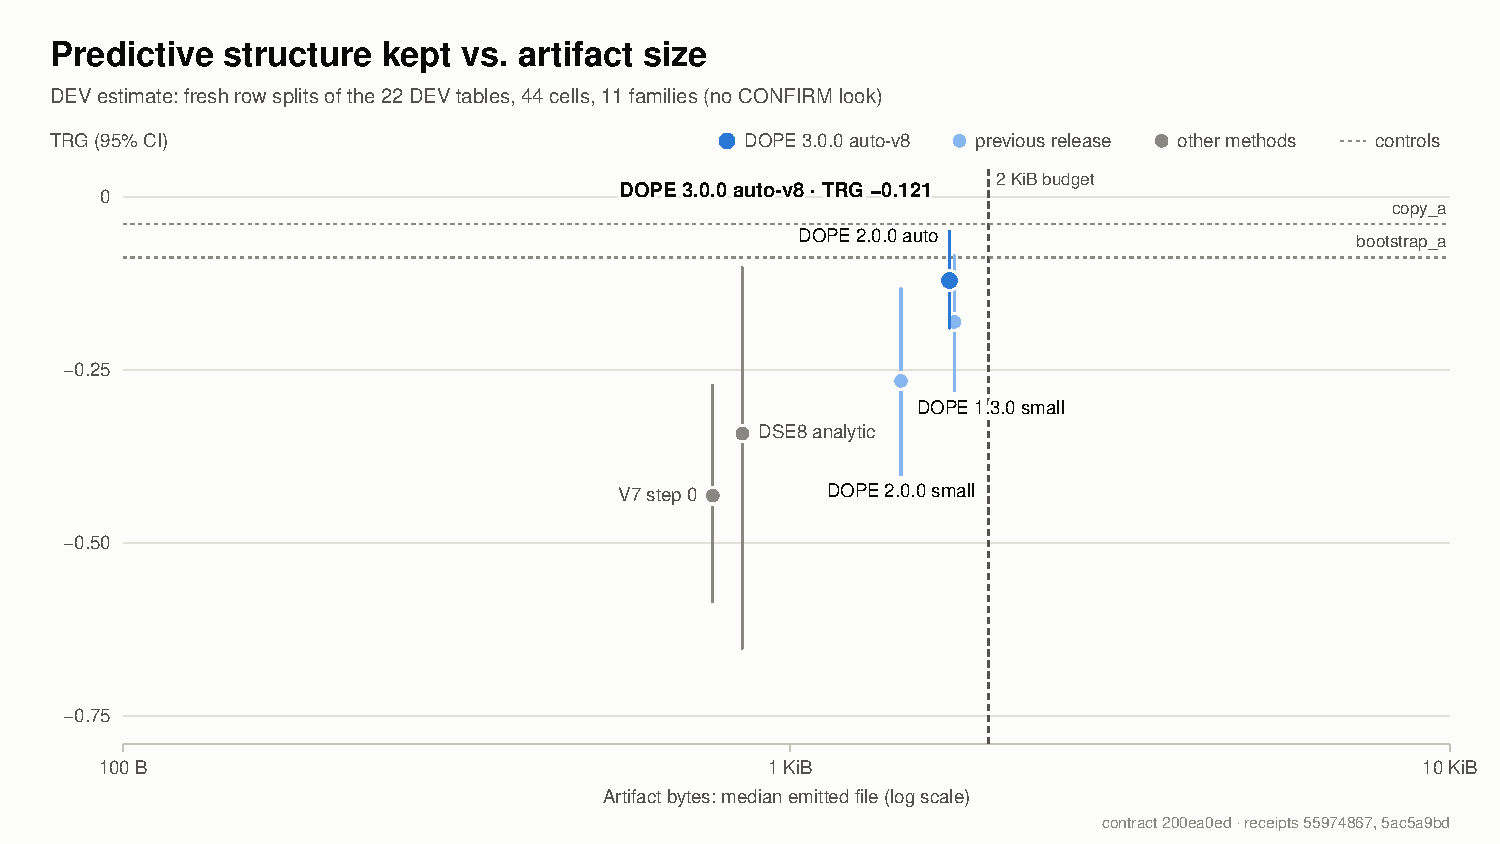
\includegraphics[width=\linewidth]{figures/hero-v3.pdf}
  \caption{TRG with its \VThree{CiLevel} family-bootstrap interval against the median file size (log axis) on the pre-registered report look (\S\ref{sec:protocol}): \VThree{CandCells} informative cells in \VThree{Families} families. The dashed line is the \VThree{BudgetBytes}-byte budget; dotted lines are the copy and bootstrap controls of $A$. This is the README figure, written by \texttt{dope\_kpi render-hero} from the receipts (SHA-256 prefixes \texttt{\VThree{PrimarySha}}, \texttt{\VThree{CompareSha}}) and converted to PDF without change (source SVG \texttt{\VThree{HeroSvgSha}}). The third-party generators are not in the README figure; Tables~\ref{tab:arms} and~\ref{tab:methods} report them.}
  \label{fig:hero}
\end{figure}

Much of the demand for synthetic tabular data is downstream: a model is trained on synthetic rows and then used on real ones.
DOPE treats this as a compression problem.
A table with a declared target is the input to a compiler; its output is an artifact of at most $B$ bytes that stores no source rows, and a sampler draws rows from the artifact alone.
The question each release answers is how much of the table's predictive structure survives at a fixed byte budget, measured by learners that never see the source rows during training.

Earlier releases offered two encoders under a common container: the Format~1 program~\citep{dope2026v1} and, in release~\VThree{BaseVersion}, a per-table choice between Format~1 and the V7 single-encoding packet~\citep{dope2026v2}.
Release~\VThree{ReleaseVersion} replaces the second candidate with \texttt{DSE8}, an analytic packet that needs no trained weights, and adds the encoder \cli{-{}-format auto-v8}, which chooses per table between Format~1 and \texttt{DSE8} with a duplicate-grouped two-fold check on the fitting rows.
The whole file, header included, stays within the budget (\VThree{BudgetBytes}~bytes by default).

\paragraph{Contributions.}
\begin{enumerate}
  \item \textbf{A packet codec with an explicit byte model} (\S\ref{sec:codec}, Appendix~\ref{app:codec}). \texttt{DSE8} is a CRC-checked sequence of tagged sections. Mandatory sections are sized by a closed-form byte model before fitting; optional sections are appended in a fixed order and truncated to the longest prefix that fits. Decoding is row-local and counter-seeded, so row $i$ depends only on the artifact, the seed and $i$.
  \item \textbf{An analytic, weight-free fit of that packet from the fitting rows only} (\S\ref{sec:fit}): typed marginals clipped at a support floor, a low-rank factor copula with regimes, and a calibrated target head with gated effects, pairwise interactions and oblivious trees.
  \item \textbf{Per-table codec selection} (\S\ref{sec:select}): \cli{auto-v8} keeps \texttt{DSE8} only when it beats Format~1 by a margin on a target-stratified, duplicate-grouped two-fold check and loses little on each fold.
  \item \textbf{A FIT-only evidence bank} (\S\ref{sec:evidence}): a deterministic, layout-frozen summary of the fitting rows that is invariant to row order and equivariant to column order, built to train learned encoders without per-table caching or access to evaluation rows.
  \item \textbf{A complete account of one pre-registered evaluation} (\S\S\ref{sec:protocol}--\ref{sec:results}), including the guards that fail, a sign-flip calibration of the decision rule and four third-party generators scored under the same protocol. Every number in this paper is rendered from committed receipts and checked in continuous integration (\S\ref{sec:repro}).
\end{enumerate}

\paragraph{What we do not claim.}
The evaluation is a development-set estimate; no confirmation, holdout or sealed panel was opened.
The comparison against the previous encoder improves TRG but its outcome under the contract is \VThree{Outcome}, not PROMOTE.
The artifacts do not make synthetic rows realistic in the two-sample sense, and the privacy diagnostics are empirical audits, not guarantees.
Section~\ref{sec:limits} lists these limitations in full.

\section{Related work}\label{sec:related}

\paragraph{Tabular generative models.}
Gaussian-copula synthesizers combine per-column marginals with a dependence model~\citep{sklar1959fonctions,patki2016sdv}.
CTGAN and TVAE fit conditional adversarial and variational models with mode-specific normalization~\citep{xu2019ctgan}; adversarial random forests alternate between a forest discriminator and a density estimate on its leaves~\citep{watson2023arf}; TabDDPM and TabSyn are diffusion models, the latter in a learned latent space~\citep{kotelnikov2023tabddpm,zhang2024tabsyn}.
These methods are designed for fidelity at whatever model size the data needs.
DOPE fixes the artifact size instead and asks how much downstream utility survives at that size.
We score SDV's Gaussian copula, CTGAN and TVAE and the ARF of arfpy under the same protocol, with their library defaults and no byte budget (\S\ref{sec:results}).

\paragraph{Dataset distillation and coresets.}
Dataset distillation learns a few synthetic examples on which a model trains well~\citep{wang2018distillation}, and coresets select weighted subsets whose loss approximates the full data's~\citep{bachem2017coresets,mirzasoleiman2020craig}.
Both store examples, real or synthetic, and are budgeted in examples.
A DOPE artifact stores a parametric generator and no rows, and is budgeted in bytes of the whole file.

\paragraph{Utility, realism and privacy metrics.}
Train-on-synthetic, test-on-real (TSTR) scores a generator by the test loss of a model trained on its samples~\citep{esteban2017tstr}.
TRG (\S\ref{sec:protocol}) is a TSTR variant that normalizes by a train-on-real reference and subtracts the same quantity for a second real sample of equal size, so that zero means ``as useful as fresh real data''.
Classifier two-sample tests (C2ST) measure whether synthetic and real rows can be told apart~\citep{lopezpaz2017c2st}; sample-level fidelity and coverage metrics refine this view~\citep{alaa2022faithful}.
Differential privacy gives formal guarantees~\citep{dwork2006calibrating}; synthetic data without such a mechanism can still leak membership~\citep{shokri2017membership,stadler2022groundhog}.
Our privacy gates are distance- and attack-based audits of that kind, not guarantees.

\paragraph{Statistical protocol.}
Intervals come from a bootstrap~\citep{efron1979bootstrap} that resamples lineage families, the cluster bootstrap of \citet{davison1997bootstrap}; comparisons use Holm's step-down adjustment~\citep{holm1979simple}.
The decision rule and comparison were fixed before the reported look~\citep{nosek2018preregistration}.
Because the same development tables were used for selection, the look is subject to the adaptive-reuse concerns studied by \citet{dwork2015reusable} (\S\ref{sec:limits}).

\section{The release encoder}\label{sec:method}

\paragraph{Setting.}
The input is a table $D_{\mathrm{fit}}$ of $n$ rows with $p$ feature columns and a declared target $y$; the task is regression, binary or multiclass classification with $K$ classes.
The encoder writes one artifact $a$ with $|a|\le B$, where $|a|$ counts every byte of the file and $B=\VThree{BudgetBytes}$ by default.
The sampler reads $a$ and a seed and emits rows $(\tilde x,\tilde y)$ in the raw column space.
Every statistic in $a$ is computed from $D_{\mathrm{fit}}$ alone; nothing is fitted on evaluation rows.

\subsection{Container and the two candidates}\label{sec:container}
Every \cli{auto-v8} artifact is a \texttt{DPA1} container: a \VThree{DpaHeaderBytes}-byte header holding a magic, an encoder tag and a weights fingerprint (all zero when no learned weights are needed), followed by the payload.
The payload is one of two candidates fitted on all of $D_{\mathrm{fit}}$:
\begin{itemize}
  \item \textbf{Format~1}, a compressed program~\citep{dope2026v1}: a safetensors file holding one compressed stream with quantile marginals on a normal-score grid, a regime mixture of Gaussian copulas, and a target model made of a residual network and boosted oblivious trees, with bit depths chosen by a rate--distortion search. It is fitted within $B-\VThree{DpaHeaderBytes}$ bytes.
  \item \textbf{\texttt{DSE8}}, preceded by a compact column-schema section (types and level names needed to write raw rows) and fitted within the room that remains. If the schema leaves fewer than \VThree{MinPacketRoom}~bytes, \cli{auto-v8} writes Format~1 directly.
\end{itemize}

\subsection{The \texttt{DSE8} packet and its byte accounting}\label{sec:codec}
A \texttt{DSE8} packet is a \VThree{DseHeaderBytes}-byte header, a sequence of sections in ascending tag order, each framed by a \VThree{TlvBytes}-byte tag-and-length prefix, and a \VThree{CrcBytes}-byte CRC32 over all preceding bytes (Table~\ref{tab:bytes}; header fields in Appendix~\ref{app:codec}).
For a file written by \cli{auto-v8} with \texttt{DSE8} chosen,
\begin{equation}\label{eq:bytes}
  |a| \;=\; D + s + H + C + \sum_{\text{sections } j} \bigl(T + \ell_j\bigr) \;\le\; B ,
\end{equation}
where $D$, $H$, $T$ and $C$ are the fixed sizes of Table~\ref{tab:bytes}, $s$ is the schema section and $\ell_j$ the payload of section $j$.

\begin{table}[t]
  \centering\small
  \caption{Byte accounting of a \texttt{DSE8} file. Fixed sizes and the planner's byte model are read from the Rust sources by the paper renderer; $p$ active columns ($p\le\VThree{MaxCols}$), copula rank $r\le\VThree{MaxRank}$, $\kappa\le\VThree{KnotCount}$ quantile knots, $o=K$ outputs for multiclass targets and $o=$ one output otherwise.}
  \label{tab:bytes}
  \begin{tabular}{@{}lll@{}}
    \toprule
    Component & Bytes & Content \\
    \midrule
    \texttt{DPA1} header ($D$) & \VThree{DpaHeaderBytes} & magic, encoder tag, weights fingerprint \\
    Column schema ($s$) & variable & column types and level names (shorter with \cli{-{}-anonymize}) \\
    \texttt{DSE8} header ($H$) & \VThree{DseHeaderBytes} & task, $K$, $p$, flags, $r$, $\kappa$, quantized scalars \\
    Section frame ($T$), per section & \VThree{TlvBytes} & tag and payload length \\
    \midrule
    \emph{Mandatory sections} & & \\
    Scale card & variable & target location and scale or class ids; per column a kind, centre and scale \\
    Marginals & $p\,(\VThree{MargBaseBytes}+\kappa)$ + typed tails & kind, missing rate, range, $\kappa$ knots; lattice or atom tails \\
    Copula loadings & $p\,r$ & one signed byte per loading \\
    Target head & $\VThree{LinFixedBytes} + o\,(\VThree{LinPerOutBytes}+p)$ & temperature; per output a scale, an intercept, $p$ signed weights \\
    Nominal groups & variable & one-hot groups with level probabilities, when present \\
    \midrule
    \emph{Optional sections, in this order} & & \\
    Regimes & variable & mixture weights and factor means \\
    Main effects & \VThree{EffectBytes} each, at most \VThree{MaxEffects} & column, output, scale, \VThree{EffectBins} binned values \\
    Pair interactions & \VThree{PairBytes} each, at most \VThree{MaxPairs} & column pair, output, product and XOR weights \\
    Oblivious trees & \VThree{TreeBytes} each, at most \VThree{MaxTrees} & depth \VThree{TreeDepth}: split columns and thresholds, scale, \VThree{TreeLeaves} leaves \\
    Residual model & variable & regression only: heteroscedastic weights, quantile shifts \\
    \midrule
    CRC32 trailer ($C$) & \VThree{CrcBytes} & over every preceding byte \\
    \bottomrule
  \end{tabular}
\end{table}

\paragraph{Planning and packing.}
Before fitting, a planner picks the active columns $p$, the knot count $\kappa$ and the rank $r$ so that the mandatory sections, estimated with the byte model of Table~\ref{tab:bytes}, leave room for optional sections; columns beyond the $p$ active ones are not modelled, and the sampler writes their stored median.
After fitting, the packer writes the mandatory sections and then each optional section in the fixed order of Table~\ref{tab:bytes}.
Effects, pairs and trees are ordered by fitted utility, and the packer keeps the longest prefix of each list that still fits, so a packet can be truncated to a smaller budget by dropping trailing items without refitting.
If the mandatory sections alone exceed the room, the fit is retried with a smaller planning budget; a candidate that never fits is not produced.

\paragraph{Decoding.}
Row $i$ of seed $\sigma$ is decoded from counter-based random streams keyed by $(\sigma, i, \text{stream}, \text{coordinate})$, so rows are independent, reproducible and can be generated in any order or in parallel.
The generative model is a factor copula:
\begin{align}
  f &\sim \mathcal N(0, I_r)\ \text{(optionally shifted by a sampled regime)}, &
  z_j &= L_j^\top f + \sigma_j \varepsilon_j, &
  x_j &= Q_j\bigl(\Phi(z_j)\bigr),
\end{align}
with loadings $L_j$, noise scales $\sigma_j$ and monotone quantile functions $Q_j$ given by the marginal knots and typed tails (lattice steps, atoms, zero inflation, missingness).
One-hot nominal groups are decoded jointly from their level probabilities, tilted by the latent scores: in each decoded row at most one indicator of a group is active, with all zero when the group's omitted baseline level is drawn.
The target is drawn last from logits
$\eta = b + W x + \sum_e g_e(z) + \sum_q h_q(z) + \sum_t \mathrm{tree}_t(z)$
of the linear head, the main effects, the pair interactions and the oblivious trees: a softmax or logistic draw at a fitted temperature for classification, and for regression the head's mean plus noise whose scale may depend on $z$ and whose quantiles are shifted by the residual section.

\subsection{Analytic fit from the fitting rows}\label{sec:fit}
The released encoder fits \texttt{DSE8} without learned weights.
\begin{enumerate}
  \item \textbf{Scale card and typed marginals.} Column kinds (continuous, lattice, discrete atoms, zero-inflated, constant) are inferred from $D_{\mathrm{fit}}$. Each column's encoded range runs between its empirical quantiles at levels $u$ and $1-u$, where $u=\min(\VThree{TailCap},\,k/\max(n_{\mathrm{obs}}+1,\VThree{TailMinDen}))$ for $n_{\mathrm{obs}}$ observed values and support floor $k=\VThree{SupportK}$; discrete values that occur at least $k$ times may instead be encoded as atoms, depending on the column's type.
  \item \textbf{Copula.} Rank-$r$ loadings are fitted to tie-aware normal scores, with loading norms capped below one so that every column keeps its own noise; a small mixture of factor means (regimes) is fitted when the budget allows.
  \item \textbf{Target head.} Ridge-penalized Newton (IRLS) fits the linear head, with the penalty chosen by out-of-fold cross-validation and the logit temperature calibrated out of fold.
  \item \textbf{Gated residual boosting.} Main effects, pairwise product and XOR interactions, and depth-\VThree{TreeDepth} oblivious trees are fitted in that order on the working residual. Because the decoder evaluates them on latent scores $z$, each real value is binned by the interval of $z$ that its tie group occupies, so fitting and decoding see the same bins. A component is kept only if it lowers a proper loss~\citep{gneiting2007strictly} on a deterministic inner validation split.
  \item \textbf{Intercept calibration.} After packing, the encoder decodes a fixed probe of synthetic feature rows from the packet itself and solves for intercepts so that the mean predicted class probabilities (for regression, the mean prediction) on those rows match the fitting rows. This corrects the shift between the real $x$ the head was fitted on and the synthetic $x$ it is applied to.
\end{enumerate}

\subsection{Per-table selection (\cli{auto-v8})}\label{sec:select}
Format~1 and \texttt{DSE8} are both fitted on all of $D_{\mathrm{fit}}$; a check on $D_{\mathrm{fit}}$ decides which one is written.
Rows are grouped into exact-duplicate groups over the feature and target columns.
If there are fewer than $G=\VThree{MinCheckGroups}$ groups, Format~1 is written (or \texttt{DSE8} if Format~1 does not fit).
Otherwise the groups are shuffled, ordered by target value for classification, and dealt alternately into halves $H_1, H_2$, so no duplicate group straddles the halves and class proportions are balanced.
On fold $f$, each candidate is refitted on one half, $\VThree{CheckSynthFactor}$ times as many rows as that half are sampled from it, and two internal auditors (a linear model and gradient-boosted trees) are trained on the sample and on the real half and scored on the other half.
The candidate's fold score $s^{(f)}$ is the minimum over auditors of the retention $(L_0-L_{\mathrm{syn}})/(L_0-L_{\mathrm{real}})$, with $L_0$ the null loss; if a classification fold has fewer than \VThree{MinTestPerClass} test rows in some class, the check is void and Format~1 is kept.
With fold means $\bar s$, \texttt{DSE8} is written if and only if
\begin{equation}\label{eq:select}
  \bar s_{\texttt{DSE8}} > \bar s_{\mathrm{F1}} + \delta
  \quad\text{and}\quad
  s^{(f)}_{\texttt{DSE8}} \ge s^{(f)}_{\mathrm{F1}} - \nu \ \text{ for both folds } f,
  \qquad \delta=\VThree{SelectionMargin},\ \nu=\VThree{FoldVeto}.
\end{equation}
The margin $\delta$ is the constant that \cli{-{}-format auto} also uses; the per-fold veto $\nu$ stops one favourable fold from carrying the decision.
When learned \texttt{DSE8} weights are supplied (\cli{-{}-v8-weights}), a third, neural candidate enters the same rule and must beat both others by $\delta$; the release ships no such weights, so by default \cli{auto-v8} chooses between Format~1 and the analytic packet only.

\section{Describing a table}\label{sec:features}

A compact generator has to decide which features of a table are worth encoding. Ties and atoms matter when a sampler must stay on the right support. A large residual after an additive fit can justify spending bytes on interactions. Strong class imbalance may make a fold or a proposed sample uninformative. These are properties of the fitting split and its declared task, so we recompute them whenever that split changes.

\subsection{Fitting-only evidence}

The evidence bank records named statistics by column, pair, class, feature group, and table. Its shape depends on the schema, and each coordinate has a validity mask. A measured zero and an unavailable measurement therefore have different representations. Appendix~\ref{app:evidence} gives the frozen layout and support rule.

\begin{table}[!htbp]
  \centering
  \small
  \begin{tabularx}{\linewidth}{@{}p{0.23\linewidth}X@{}}
    \toprule
    Evidence & Measurements \\
    \midrule
    Support and shape & Ties, supported atoms, lattice structure, quantile residuals, missingness, and tail summaries. \\
    Dependence and target & Tie-aware associations, factor structure, class summaries, out-of-fold residual structure, and pairwise effects. \\
    Learner witnesses & Out-of-fold linear and boosted-tree gain, grouped permutation importance, interaction energy, and calibration. \\
    Candidate diagnostics & When a packet is supplied, compare decoded rows with fitting rows using a discriminator, dependence gaps, proximity to records, and packet size. \\
    \bottomrule
  \end{tabularx}
  \caption{What the evidence bank measures. Row-derived inputs come from the fitting split. Candidate diagnostics also use rows decoded from the packet.}
  \label{tab:evidence-families}
\end{table}

The release's analytic fit uses the shared ordering and support primitives and estimates the quantities stored by each codec. The learned refinement pilot consumes the evidence tensors. A separate landmark panel can be used to diagnose a table or a synthetic draw. The default \cli{dope fit} route does not run that panel.

\subsection{Landmarks and their uses}

A landmark is the result of a small learning experiment~\citep{pfahringer2000landmarking}. Within the fitting split, train a fixed recipe on each fold's training rows and score it on that fold's validation rows. Use the fold's training rows to fit preprocessing and the constant predictor. A missing, unsupported, or unstable result remains visible as such.

A panel of recipes is more informative than a single accuracy estimate. Comparing a shaped additive fit with a tree can indicate where interactions deserve inspection. Comparing the full fit with a single-feature fit can reveal concentration of predictive signal. These contrasts are diagnostic: correlated features, finite samples, and the inductive biases of the recipes can produce large contrasts even when the underlying mechanism is simple. They do not establish that the same drivers are preserved for a different model family.

The release's codec selector uses a related idea with a different purpose. It fits and samples each candidate on fitting-only folds and checks how well fixed auditors transfer to the other fold. It uses the comparison to choose a packet before the external test rows are opened (\S\ref{sec:select}).

\subsection{How this differs from an in-context predictor}

TabPFN's technical report describes a predictor that embeds cells using, among other inputs, Fourier features and ranks computed against the column's training values. Kumo Tabular embeds cells, builds row representations with column- and row-wise attention, and predicts queries from labeled context~\citep{priorlabs2026tabpfn,nvidia2026kumotabular}. They can run within the owner's boundary, subject to the deployment setting.

DOPE summarizes the fitting split before fitting a per-table generator. The receiver needs the artifact to sample, and can choose a learner afterward. One possible composition is to use synthetic rows as context for an in-context predictor. The benchmark in this report evaluates linear, boosted-tree, and MLP learners. Transfer to an in-context model remains unmeasured.

\section{Evaluation protocol}\label{sec:protocol}

All results come from \texttt{dope\_kpi} (\path{engine/dope-arena}) under the contract \VThree{ContractId} (\path{contracts/dope-kpi.json}, SHA-256 prefix \texttt{\VThree{KpiContractSha}}), which fixes the statistic, the interval, the decision rule and its guards.
The contract's status is ``\VThree{ContractStatus}'' and it is not frozen.

\paragraph{Cells and roles.}
A cell is one table with one row split into disjoint roles: $A$, the rows a generator sees; $B$, a real twin with as many rows as $A$; $C$, calibration rows; and $T$, held-out test rows.
No duplicate group straddles two roles.
An arm fits on $A$ and emits a synthetic sample $S$ of $m\,|A|$ rows; the headline multiplier is $m=\VThree{PrimaryMult}$ and a matched-size statistic with $m=\VThree{MatchedMult}$ is reported beside it.
Tables belong to lineage families (tables from one source), each assigned to one task.

\paragraph{Retention and the twin-referenced gap.}
An auditor is a fixed learning recipe.
Fitted on rows $x$ and scored on $T$ with loss $L_x$, it has retention
\begin{equation}\label{eq:retention}
  R_x = \frac{L_{\mathrm{null}} - L_x}{L_{\mathrm{null}} - L_A},
\end{equation}
where $L_{\mathrm{null}}$ is the loss of the null prediction and $L_A$ that of the auditor fitted on $A$.
For a scored entry (cell, auditor, sample seed),
\begin{equation}\label{eq:entry}
  v = \operatorname{clip}\bigl(R_S,\ \VThree{ClipLow},\ \VThree{ClipHigh}\bigr) - R_B ,
\end{equation}
and $v=\VThree{FailedValue}$ for an entry that was not scored (a failure, an artifact over budget, a single-class sample or an unsupported table).
Values are averaged over sample seeds; a cell takes the minimum over the two statistic auditors (a seeded linear model and gradient-boosted trees); cells are averaged within a family, families within a task, and the tasks present are averaged with equal weight:
\begin{equation}\label{eq:trg}
  \TRG = \frac{1}{|\mathcal T|}\sum_{t\in\mathcal T}\frac{1}{|\mathcal F_t|}\sum_{f\in\mathcal F_t}\frac{1}{|\mathcal C_f|}\sum_{c\in\mathcal C_f}\ \min_{a}\ \bar v_{c,a}.
\end{equation}
Zero means that the synthetic rows train the auditors as well as a real twin the size of the fitting split; higher is better. We rank generators by the \emph{Transfer Score} $\VThree{ScoreScale}\times(1+\mathrm{TRG})$ in points, as the README does. It is a fixed relabel of TRG, so ranks, the Holm test and every decision are unchanged and intervals scale by \VThree{ScoreScale}. A score of \VThree{ScoreScale} is the real twin; on the report look the copy control of $A$, which returns the fitting rows themselves, scores \VThree{CopyAScorePoint}. Only at $m=\VThree{MatchedMult}$ do the synthetic sample and the twin have the same size.
A third auditor, a seeded MLP, is aggregated the same way, held out of the statistic and read only by a guard.
A (cell, auditor) unit enters only if it is informative on real data alone: the auditor fitted on $A$ must beat the null on $T$ by a material margin with a positive bootstrap lower bound, and the twin's retention must be close to one.

\paragraph{Uncertainty.}
Intervals come from a stratified family bootstrap: each of \VThree{BootDraws} draws resamples the families of every task with replacement and recomputes Eq.~\eqref{eq:trg}.
The \VThree{CiLevel} interval runs between the draws at the \VThree{LowerPct}th and \VThree{UpperPct}th percentiles, and the one-sided $p$ for a paired difference $\Delta\le 0$ is the share of draws at or below zero, with one added to numerator and denominator.
Both arms of a comparison read the same draws.

\paragraph{Decision rule.}
A comparison pairs a candidate with a baseline on their common cells and bootstraps the per-family differences.
Holm's adjustment runs over the comparisons of one receipt.
The outcome is PROMOTE if and only if
(i)~the interval's lower bound is above \VThree{CiLowGt};
(ii)~the Holm-adjusted $p$ is below \VThree{HolmAlpha};
(iii)~$\Delta \ge \max(\VThree{MinDelta}, \text{noise s.d.})$; and
(iv)~every guard passes: each task's lower bound is above \VThree{TaskCiLowGt}; the held-out MLP difference is at least \VThree{MlpDeltaGe}; the realism and privacy coverage differences are above \VThree{RealismDeltaGt} and \VThree{PrivacyDeltaGt}; the candidate's exact-copy excess is at most \VThree{CopyLe}; and every produced file is within the \VThree{BudgetBytes}-byte budget.
It is REJECT if the interval's upper bound is below zero, and HOLD otherwise.
Coverage is the share of informative statistic entries whose synthetic file passes a realism (or privacy) gate, aggregated like the statistic.
The realism gate bounds the C2ST AUC of a boosted-tree discriminator between $B$ and $S$, the per-column marginal AUC and the rule-violation ratio; the privacy gate bounds a distance-to-closest-record share, a distance-based membership-inference AUC and its true-positive rate at a low false-positive rate, and requires the declared support floor.
Appendix~\ref{app:guards} gives the thresholds and the exact-copy excess.

\paragraph{Calibration of the rule.}
Each comparison also carries a sign-flip null: in each of \VThree{NullReplicates} replicates every family's paired differences are multiplied by an independent fair sign and the rule is reapplied.
The receipt reports the false-PROMOTE rate of the statistical conditions (i)--(iii) alone and of the conditions together with the guards a flip can move, each with a Wilson interval; the contract deems a rate of at most \VThree{NullMaxRatePct} acceptable.
These rates are reported beside the decision and do not enter it.

\paragraph{The look.}
Under a pause on the confirmation, holdout and sealed panels, every number in this paper comes from development (DEV) tables.
The encoder was selected on DEV in steps recorded in the scoreboard's README before each was scored: a screen on a small DEV schedule, a decision on a wider DEV schedule, and a single report on fresh row splits of the same DEV tables, planned before selection and scored once after it.
No guard, threshold or parameter was tuned on the report.
The third-party generators were fitted and scored on the same report schedule, once each, after the encoder was fixed.
The receipts identify the schedule by SHA-256 (prefix \texttt{\VThree{ScheduleSha}}) but do not include it.

\paragraph{Comparisons with the third-party generators.}
Each third-party generator is paired with DOPE on their common cells, and Holm's adjustment runs over the \VThree{MethodsHolmM} pairs.
The receipt that scored the generators (\path{compare-methods.json}) asks whether each generator improves on DOPE.
The direction reported in Table~\ref{tab:paired}, DOPE against each generator, was re-reduced after scoring from the same per-cell scores with the same \texttt{dope\_kpi} build, which reproduces the committed receipt byte for byte (\path{evidence/paper/} under the scoreboard).
The paired differences and intervals are the same numbers with the sign reversed; only the one-sided $p$-values and the guard outcomes depend on the direction.
Each re-reduced receipt applies the decision rule with Holm's adjustment over its own pair; adjusting over the \VThree{MethodsHolmM} pairs instead changes no outcome.
A second look, pre-registered before any third-party generator was scored on it, is a descriptive repeat of the comparison on other row splits of the same DEV tables with the same generator recipes, scored and reduced by the \texttt{dope\_kpi} build that had already scored DOPE there; it is reduced directly in the reported direction, with Holm's adjustment over its own \VThree{MethodsHolmM} pairs, and the existing scores of DOPE and the reference rows on those splits are reused unchanged.

\section{Results}\label{sec:results}

\begin{table}[t]
  \centering\footnotesize\setlength{\tabcolsep}{3.5pt}
  \caption{Every arm of the report look (receipt \texttt{\VThree{PrimarySha}}), with the README's rows, columns and values; the columns are wrapped into panels (a) and (b). Bytes are whole-file sizes. TRG uses the \VThree{PrimaryMult}$\times$ sample; per-task values give the number of families in parentheses. Retention medians are unclipped. C2ST is the median two-sample AUC (chance level means indistinguishable). Realism and privacy are coverage shares, and copies the exact-copy excess, mean (maximum file). Controls carry no artifact.}
  \label{tab:arms}
  % Generated by docs/whitepaper-v3/scripts/render_v3_paper.py -- DO NOT EDIT BY HAND.
% third-party baseline rows: sdv-gaussian-copula, sdv-ctgan, sdv-tvae, arfpy-arf
\textbf{(a)}\par\smallskip
\begin{tabular}{@{}llrrrrr@{}}
\toprule
Arm & Class & \makecell{Bytes median / max\\ / share $\le$ budget} & TRG [95\% CI] & \makecell{Regression\\(families)} & \makecell{Binary\\(families)} & \makecell{Multiclass\\(families)} \\
\midrule
\textbf{\texttt{dope-v3b-auto-v8}} & source\_free & 1787 / 2048 / 1.000 & \ensuremath{-}0.121 [\ensuremath{-}0.189, \ensuremath{-}0.049] & \ensuremath{-}0.137 (4) & \ensuremath{-}0.136 (3) & \ensuremath{-}0.089 (4) \\
\texttt{dope-2.0.0-auto} & source\_free & 1817.5 / 2048 / 1.000 & \ensuremath{-}0.181 [\ensuremath{-}0.280, \ensuremath{-}0.085] & \ensuremath{-}0.118 (4) & \ensuremath{-}0.278 (3) & \ensuremath{-}0.146 (4) \\
\texttt{dope-2.0.0-small} & source\_free & 1508 / 2043 / 1.000 & \ensuremath{-}0.267 [\ensuremath{-}0.402, \ensuremath{-}0.133] & \ensuremath{-}0.250 (4) & \ensuremath{-}0.438 (3) & \ensuremath{-}0.112 (4) \\
\texttt{dope-1.3.0-small} & source\_free & 1508 / 2043 / 1.000 & \ensuremath{-}0.266 [\ensuremath{-}0.399, \ensuremath{-}0.133] & \ensuremath{-}0.249 (4) & \ensuremath{-}0.438 (3) & \ensuremath{-}0.109 (4) \\
\texttt{pr390-v7-step0} & source\_free & 782.5 / 2026 / 1.000 & \ensuremath{-}0.432 [\ensuremath{-}0.585, \ensuremath{-}0.273] & \ensuremath{-}0.102 (4) & \ensuremath{-}0.545 (3) & \ensuremath{-}0.648 (4) \\
\texttt{dse8-p0-v3b} & source\_free & 867.5 / 2048 / 1.000 & \ensuremath{-}0.342 [\ensuremath{-}0.652, \ensuremath{-}0.103] & \ensuremath{-}0.094 (4) & \ensuremath{-}0.276 (3) & \ensuremath{-}0.655 (4) \\
\midrule
\texttt{sdv-gaussian-copula} & source\_free & 140675.5 / 1145929 / 0.000 & \ensuremath{-}0.598 [\ensuremath{-}0.721, \ensuremath{-}0.482] \textdagger{} & \ensuremath{-}0.168 (4) & \ensuremath{-}0.612 (3) & \ensuremath{-}1.015 (4) \\
\texttt{sdv-ctgan} & source\_free & 1053957.5 / 5404151 / 0.000 & \ensuremath{-}1.692 [\ensuremath{-}1.827, \ensuremath{-}1.552] \textdagger{} & \ensuremath{-}1.502 (4) & \ensuremath{-}1.888 (3) & \ensuremath{-}1.685 (4) \\
\texttt{sdv-tvae} & source\_free & 475125.5 / 3340780 / 0.000 & \ensuremath{-}1.039 [\ensuremath{-}1.262, \ensuremath{-}0.822] \textdagger{} & \ensuremath{-}0.700 (4) & \ensuremath{-}1.432 (3) & \ensuremath{-}0.986 (4) \\
\texttt{arfpy-arf} & source\_free & 2937782.5 / 24068428 / 0.000 & \ensuremath{-}0.228 [\ensuremath{-}0.416, \ensuremath{-}0.100] \textdagger{} & \ensuremath{-}0.071 (4) & \ensuremath{-}0.412 (3) & \ensuremath{-}0.203 (4) \\
\midrule
\texttt{twin\_c} & control & -- & \ensuremath{-}0.060 [\ensuremath{-}0.060, \ensuremath{-}0.060] & \ensuremath{-}0.074 (1) & -- & \ensuremath{-}0.046 (1) \\
\texttt{copy\_a} & control & -- & \ensuremath{-}0.039 [\ensuremath{-}0.069, \ensuremath{-}0.014] & \ensuremath{-}0.017 (4) & \ensuremath{-}0.056 (3) & \ensuremath{-}0.045 (4) \\
\texttt{bootstrap\_a} & control & -- & \ensuremath{-}0.088 [\ensuremath{-}0.147, \ensuremath{-}0.036] & \ensuremath{-}0.085 (4) & \ensuremath{-}0.039 (3) & \ensuremath{-}0.139 (4) \\
\texttt{indep\_marginals} & control & -- & \ensuremath{-}1.222 [\ensuremath{-}1.387, \ensuremath{-}1.095] & \ensuremath{-}1.135 (4) & \ensuremath{-}1.381 (3) & \ensuremath{-}1.149 (4) \\
\texttt{label\_shuffle} & control & -- & \ensuremath{-}1.164 [\ensuremath{-}1.269, \ensuremath{-}1.063] & \ensuremath{-}1.235 (4) & \ensuremath{-}1.004 (3) & \ensuremath{-}1.251 (4) \\
\bottomrule
\end{tabular}
\par\medskip\textbf{(b)}\par\smallskip
\begin{tabular}{@{}lrrrr@{}}
\toprule
Arm & \makecell{Median retention\\linear / gbdt / mlp} & C2ST & \makecell{Realism / privacy /\\copies mean (max)} & \makecell{Failed\\/ cells} \\
\midrule
\textbf{\texttt{dope-v3b-auto-v8}} & 0.942 / 0.916 / 0.792 & 0.967 & 0.194 / 0.688 / 0.000 (0.000) & 0 / 44 \\
\texttt{dope-2.0.0-auto} & 0.939 / 0.917 / 0.792 & 0.958 & 0.306 / 0.719 / 0.000 (0.001) & 0 / 44 \\
\texttt{dope-2.0.0-small} & 0.918 / 0.915 / 0.865 & 0.925 & 0.306 / 0.507 / 0.000 (0.000) & 7 / 44 \\
\texttt{dope-1.3.0-small} & 0.912 / 0.915 / 0.798 & 0.925 & 0.306 / 0.507 / 0.000 (0.000) & 7 / 44 \\
\texttt{pr390-v7-step0} & 0.896 / 0.840 / 0.728 & 0.986 & 0.194 / 0.774 / 0.000 (0.001) & 0 / 44 \\
\texttt{dse8-p0-v3b} & 0.950 / 0.942 / 0.741 & 0.977 & 0.194 / 0.753 / 0.000 (0.000) & 0 / 44 \\
\midrule
\texttt{sdv-gaussian-copula} & 0.525 / 0.510 / 0.329 & 0.992 & 0.111 / 0.601 / 0.005 (0.200) & 0 / 44 \\
\texttt{sdv-ctgan} & \ensuremath{-}0.514 / \ensuremath{-}0.425 / \ensuremath{-}0.557 & 0.996 & 0.000 / 0.743 / 0.006 (0.271) & 0 / 44 \\
\texttt{sdv-tvae} & 0.175 / 0.466 / 0.291 & 0.977 & 0.000 / 0.326 / 0.000 (0.000) & 5 / 44 \\
\texttt{arfpy-arf} & 0.906 / 0.874 / 0.835 & 0.941 & 0.278 / 0.031 / 0.000 (0.004) & 0 / 44 \\
\midrule
\texttt{twin\_c} & 0.997 / 0.993 / 0.974 & 0.522 & -- / -- / -- & 0 / 8 (36 n/a) \\
\texttt{copy\_a} & 1.000 / 1.000 / 1.000 & 0.530 & -- / -- / -- & 0 / 44 \\
\texttt{bootstrap\_a} & 0.995 / 0.995 / 0.991 & 0.572 & -- / -- / -- & 0 / 44 \\
\texttt{indep\_marginals} & \ensuremath{-}0.157 / \ensuremath{-}0.011 / \ensuremath{-}0.334 & 0.967 & -- / -- / -- & 0 / 44 \\
\texttt{label\_shuffle} & \ensuremath{-}0.105 / \ensuremath{-}0.004 / \ensuremath{-}0.208 & 0.687 & -- / -- / -- & 0 / 44 \\
\bottomrule
\end{tabular}
\par\smallskip
\parbox{\linewidth}{\raggedright \textdagger{} Scored with packets above 2048 B (the TRG reads the rows as scored): \texttt{sdv-gaussian-copula} 64 files, TRG at 2048 B \ensuremath{-}1.000; \texttt{sdv-ctgan} 64 files, TRG at 2048 B \ensuremath{-}1.000; \texttt{sdv-tvae} 45 files, TRG at 2048 B \ensuremath{-}1.000; \texttt{arfpy-arf} 64 files, TRG at 2048 B \ensuremath{-}1.000.}

\end{table}

\begin{table}[t]
  \centering\footnotesize
  \caption{The pre-registered comparison (receipt \texttt{\VThree{CompareSha}}): the README row, then each condition and guard of the decision rule with its contract threshold. Sign-flip PROMOTE is the false-PROMOTE rate of the conditions and the guards a sign flip moves (\S\ref{sec:protocol}).}
  \label{tab:compare}
  % Generated by docs/whitepaper-v3/scripts/render_v3_paper.py -- DO NOT EDIT BY HAND.
\begin{tabular}{@{}lrrrl@{}}
\toprule
Comparison & $\Delta$TRG [95\% CI] & Holm $p$ ($m$) & Sign-flip PROMOTE & Outcome \\
\midrule
\texttt{dope-v3b-auto-v8} vs \texttt{dope-2.0.0-auto} & +0.060 [+0.009, +0.114] & 0.009 (1) & 0.000 & \textbf{HOLD} \\
\bottomrule
\end{tabular}
\par\medskip
\begin{tabular}{@{}llrl@{}}
\toprule
Rule item & Threshold & Value & Check \\
\midrule
condition: interval lower bound & $>$ 0.000 & +0.009 & pass \\
condition: Holm-adjusted $p$ & $<$ 0.050 & 0.009 & pass \\
condition: minimum gain & $\ge$ +0.010 & +0.060 & pass \\
guard: tasks & $>$ \ensuremath{-}0.020 & \ensuremath{-}0.053 & \textbf{FAIL} \\
guard: mlp & $\ge$ 0.000 & \ensuremath{-}0.007 & \textbf{FAIL} \\
guard: realism & $>$ \ensuremath{-}0.030 & \ensuremath{-}0.111 & \textbf{FAIL} \\
guard: privacy & $>$ \ensuremath{-}0.030 & \ensuremath{-}0.031 & \textbf{FAIL} \\
guard: copies & $\le$ 0.005 & 0.000 (0.000) & pass \\
guard: bytes & $\le$ 2048 & 2048 & pass \\
\bottomrule
\end{tabular}

\end{table}

Figure~\ref{fig:hero} and Tables~\ref{tab:arms} and~\ref{tab:compare} report the single look of \S\ref{sec:protocol}: \VThree{Scheduled} scheduled cells, of which \VThree{Uninformative} are uninformative on real data and leave every arm, and \VThree{CandCells} informative cells in \VThree{Families} families (\VThree{RegressionFamilies} regression, \VThree{BinaryFamilies} binary and \VThree{MulticlassFamilies} multiclass).

\paragraph{Headline.}
\cli{auto-v8} reaches a TRG of \VThree{CandTrg}, against \VThree{BaseTrg} for the release~\VThree{BaseVersion} encoder, a paired gain of \VThree{Delta} with $p=\VThree{PHolm}$ (Holm over $m=\VThree{HolmM}$).
Its median file is \VThree{CandBytesMed}~bytes (\VThree{BaseBytesMed} for the baseline), the largest is \VThree{CandBytesMax}, and it fails \VThree{CandFailed} of \VThree{CandCells} cells.
The gain comes from classification: the paired task differences are \VThree{DeltaBinary} for binary and \VThree{DeltaMulticlass} for multiclass targets, and \VThree{DeltaRegression} for regression, where \cli{auto-v8} is lower on the point estimate (\VThree{CandRegression} against \VThree{BaseRegression}).

\paragraph{Matched size.}
With a synthetic sample the size of $A$ ($m=\VThree{MatchedMult}$), \cli{auto-v8} scores \VThree{CandMatched} against \VThree{BaseMatched}; the paired gain \VThree{MatchedDelta} has one-sided $p=\VThree{MatchedP}$ and its interval contains zero.
At matched size the gain is not resolved; the headline rests on the \VThree{PrimaryMult}$\times$ sample.

\paragraph{Against the other arms.}
The analytic packet used on every table, without selection (\VThree{AnalyticId}), scores \VThree{AnalyticTrg} at a median of \VThree{AnalyticBytesMed}~bytes: better than the baseline on regression (\VThree{AnalyticRegression}) but far worse on multiclass targets (\VThree{AnalyticMulticlass}).
Used alone it is worse than the baseline; within \cli{auto-v8} it is written only where the check of \S\ref{sec:select} prefers it.
The Format~1 \texttt{small} programs of releases \VThree{BaseVersion} and \VThree{OldVersion} score \VThree{PrevSmallTrg} and \VThree{OldSmallTrg} and fail \VThree{PrevSmallFailed} of \VThree{PrevSmallCells} cells, and the V7 packet with untrained decoder weights (\VThree{V7Id}) scores \VThree{V7Trg}.

\paragraph{Controls.}
Training on $A$ itself (\VThree{CopyAId}) scores \VThree{CopyATrgPoint} rather than zero: its entry value is $1-R_B$, and the minimum over auditors falls below zero whenever the twin trains one auditor better than $A$ does. A bootstrap resample of $A$ scores \VThree{BootATrgPoint}.
Both are reference points for a generator that only sees $A$.
Permuting each column independently (\VThree{IndepId}) scores \VThree{IndepTrgPoint}, and permuting only the target scores \VThree{LabelShuffleTrgPoint}.
The real-twin control from the calibration rows is applicable on only \VThree{TwinCCells} cells (\VThree{TwinCNotApplicable} lack enough rows).

\paragraph{The decision.}
Conditions (i)--(iii) hold, but \VThree{GuardsFailed} of the \VThree{GuardsTotal} guards fail (Table~\ref{tab:compare}): the regression lower bound (\VThree{GuardTasks} against a threshold of \VThree{TaskCiLowGt}), the held-out MLP difference (\VThree{GuardMlp}), realism coverage (\VThree{GuardRealism}; \VThree{CandRealism} against \VThree{BaseRealism}) and privacy coverage (\VThree{GuardPrivacy} against a threshold of \VThree{PrivacyDeltaGt}).
The exact-copy and byte guards pass.
The outcome is \textbf{\VThree{Outcome}}.

\paragraph{Calibration of the decision.}
Under the comparison's sign-flip null, the statistical conditions alone pass in \VThree{StatPassPct} of \VThree{NullReplicates} replicates (Wilson interval \VThree{StatPassLowPct}--\VThree{StatPassHighPct}), far above the contract's \VThree{NullMaxRatePct}.
With \VThree{Families} families (\VThree{RegressionFamilies}, \VThree{BinaryFamilies} and \VThree{MulticlassFamilies} per task), the percentile interval is too narrow, and the headline $p$ should be read in that light.
With the guards a flip can move, the rate is \VThree{FlipRatePct} (upper Wilson bound \VThree{FlipHighPct}): the guards, not the interval, are what keep the rule calibrated on this panel.

\section{Using a fitted artifact}\label{sec:practical}

There are three distinct steps in a deployment. First, declare the target and split real rows by duplicate group. Fit locally under a whole-file budget, using only the fitting split to choose the codec. Second, reload the artifact in another process and generate a training CSV with a recorded row count and seed. Third, fit the same downstream recipe on real fitting rows and on synthetic rows, and score both on the same withheld real rows. A null model fitted on the real fitting set anchors the retention calculation in Eq.~\eqref{eq:retention}. This gives a useful application check even without the real twin required to compute Transfer Score.

For storage or exchange, the per-table file is independent of the original runtime process. A change to the task, schema, or budget calls for a new fit. The artifact contains schema and fitted summaries, and synthetic rows can also carry information about the source. Decide whether either may cross the data boundary under the same policy that governs other derived data. This paper measures some of that risk empirically in Appendix~\ref{app:guards}.

The \href{https://github.com/neverhuman/dope#quick-start}{signed-engine quick start} demonstrates fitting, cold-process sampling, and evaluation on a deterministic fixture. The \href{https://github.com/neverhuman/dope/blob/main/docs/getting-started.md}{own-data walkthrough} covers the signed codec's sampling route and shows how to evaluate the resulting CSV.

\section{Limitations}\label{sec:limits}

\paragraph{The decision is HOLD.}
The pre-registered comparison improves TRG but does not meet the contract: \VThree{GuardsFailed} of \VThree{GuardsTotal} guards fail.
(i)~\emph{Regression.} The regression difference is \VThree{DeltaRegression}; its lower bound \VThree{GuardTasks} is below the \VThree{TaskCiLowGt} guard, and the point estimate favours the baseline.
(ii)~\emph{Held-out MLP.} The MLP auditor, which plays no part in selection or in the statistic, prefers the baseline (difference \VThree{GuardMlp}; TRG \VThree{CandMlp} against \VThree{BaseMlp}).
(iii)~\emph{Realism coverage.} The difference is \VThree{GuardRealism}: the share of informative entries whose synthetic file passes the realism gate is \VThree{CandRealism} against \VThree{BaseRealism}.
(iv)~\emph{Privacy coverage.} The difference is \VThree{GuardPrivacy}, just below the \VThree{PrivacyDeltaGt} guard (\VThree{CandPrivacy} against \VThree{BasePrivacy}).
We have not established the causes of these failures, and \cli{-{}-format 1} remains the command-line default.

\paragraph{Realism.}
The median C2ST AUC of \cli{auto-v8} is \VThree{CandC2st}; the baseline's is \VThree{BaseC2st} and that of independently permuted columns is \VThree{IndepC2st}, while real resamples score \VThree{CopyAC2st} (copy of $A$) and \VThree{BootAC2st} (bootstrap of $A$).
A boosted-tree discriminator separates these rows from real ones about as easily as rows with no dependence at all.
The artifacts preserve predictive structure for the auditors far better than permuted columns do (TRG \VThree{CandTrgPoint} against \VThree{IndepTrgPoint}), but they are not realistic samples, and nothing here supports using them where realism matters.

\paragraph{Privacy.}
Storing no source rows and clipping marginals at a support floor are design properties, not guarantees.
The privacy gate is an empirical audit (distance to closest record, a distance-based membership-inference attack, exact copies) on the rows scored; it is neither differential privacy~\citep{dwork2006calibrating} nor HIPAA de-identification, and passing it does not rule out other attacks~\citep{stadler2022groundhog}.

\paragraph{Development data only.}
No confirmation, holdout or sealed panel was opened.
Both looks used fresh row splits, but of the same DEV tables on which the encoder was designed and selected, so they say little about tables or lineages outside that set; adaptive reuse of a development set biases such estimates upward~\citep{dwork2015reusable}.
The pre-registration and its hash log are committed with the receipts; the schedules are identified in the receipts by hash and not published.

\paragraph{Small panel and an unfrozen contract.}
The report look has \VThree{Families} informative families, as few as \VThree{BinaryFamilies} in one task.
The sign-flip null shows that the percentile interval is anti-conservative at this size (\S\ref{sec:results}), Holm's adjustment covers a single comparison, and the matched-size gain is not resolved.
The contract is a candidate and not frozen, so the rule itself may change before a confirmatory look.

\paragraph{The final look.}
The final look has the same limits, with \VThree{FlFamilies} informative families, and on it the rule is not calibrated.
Neither look shows the released engine improving on release~\VThree{BaseVersion} under the contract; the candidate's PROMOTE rests on \VThree{FlNonzeroFamilies} families and did not change what shipped.

\paragraph{Third-party baselines.}
Each third-party generator was fitted once per cell on this development look, with library defaults, no tuning and no byte cap (files scored up to \VThree{MethodsScoreBudget}~bytes), so it fails the byte guard by construction; its TRG reflects its own file sizes.
Entries whose sample holds a single class score \VThree{FailedValue} by protocol; the run's report (\path{methods-report.md}) attributes TVAE's failed cells to such samples.
The comparisons are between these configurations on these splits, not the methods in general; SDV and its libraries are licensed \VThree{SdvLicense} and arfpy \VThree{ArfpyLicense}.

\paragraph{Provenance.}
The receipts record \texttt{dope\_kpi} \VThree{ToolVersion} with build commit ``\VThree{ToolGitSha}'', and the scored packets are not committed, so the scores cannot be recomputed from the repository alone.
The scoreboard's README reports that a local build of the release source reproduced every scheduled packet's SHA-256 and that the signed binary must too; no committed receipt records either, so we do not claim that the released binary reproduces every scored packet.

\section{Reproducibility}\label{sec:repro}

\paragraph{From receipts to this paper.}
Three links, each checked by a tool rather than by hand:
\begin{enumerate}
  \item \texttt{dope\_kpi primary} and \texttt{compare} write the receipts \path{bench/real-world/results/scoreboard/v3.0.0/primary.json} and \path{compare.json} (SHA-256 prefixes \texttt{\VThree{PrimarySha}} and \texttt{\VThree{CompareSha}}): sorted-key JSON that records the SHA-256 of the contract, the schedule and every rows file read.
  \item \texttt{dope\_kpi render-readme} and \texttt{render-hero} turn those receipts into the README block and hero figure; \path{render-manifest.json} records their SHA-256s and \path{tools/claims/dope1.py --check} refuses drift.
  \item \path{docs/whitepaper-v3/scripts/render_v3_paper.py} writes every \texttt{\textbackslash VThree} macro and results table from the receipts, the contracts and constants parsed from the Rust sources, and fails unless every release row equals the README block's; it converts the hero SVG to PDF and records both SHA-256s. Third-party rows come from \path{primary-methods.json} and \path{compare-methods.json}, which must repeat the release receipts' run and arms and agree with the run's \path{MANIFEST.json}; Appendix~\ref{app:arms} lists the final look's checks.
\end{enumerate}

\paragraph{What continuous integration checks.}
\texttt{render\_v3\_paper.py -{}-check} fails on drift of a generated file or the hero PDF, an undefined macro, a typed claim the receipts no longer support, or a digit typed outside a macro, citation, label or short allowlist.
The \texttt{paper-clean} job rebuilds the generated files and PDF with fixed timestamps and requires a zero diff; \path{docs/whitepaper-v3/README.md} lists the commands.

\section{Conclusion}\label{sec:conclusion}

A byte budget forces a generator to choose which structure to keep. On the development tables studied here, the signed release preserved more measured predictive utility than storing and resampling fitting rows under the same cap. Against uncapped library defaults, its report point estimate leads the other generators and its file is smaller. The paired comparisons support a difference against the SDV configurations on these split sets. The comparison with ARF remains uncertain.

The resulting artifact is a task-specific way to generate training data. Its value should be judged on a learner and test split relevant to the proposed use, alongside disclosure and realism constraints. An independent confirmation panel and transfer to additional learner families would test whether the pattern extends beyond the present development tables.


\bibliographystyle{plainnat}
\bibliography{references-v3}

\appendix
\section{\texttt{DSE8} wire format}\label{app:codec}

\paragraph{Header.}
The \VThree{DseHeaderBytes}-byte header holds, in order: the magic \texttt{DSE8}, the format version, the task, the class count $K$, the active column count $p$, the raw column count, a flag byte, the copula rank $r$, the knot level $\kappa$, the quantized logarithm of the fitting-row count, the latent clip $z_{\max}$, the residual scale, the positive-class prior, the inverse degrees of freedom $1/\nu$ of a row-level Student-$t$ scale on the factors (zero for Gaussian factors), the section count, the code tier and a reserved field.
The flags mark a normalized-only packet, a column map, custom class ids, stored medians of dropped columns, skew-$t$ factors, and a neural encoder.

\paragraph{Sections.}
Tags ascend in this order: scale card, marginals, copula, linear head, nominal groups, regimes, main effects, pair interactions, oblivious trees, residual model, neural code, weights fingerprint.
The scale card (absent only in the normalized-only mode), marginals, copula and linear head are always present, and nominal groups are present whenever the table has one-hot groups, since dropping them would let the sampler emit rows with zero or several active levels.
The neural code and the weights fingerprint appear only in neural packets.
Quantization is per section: loadings, effect bins, pair weights, regime means and tree leaves are signed bytes with a fixed or stored scale; marginal ranges and effect scales are half-precision floats; scale-card centres are single-precision and scales brain-float; probabilities are unsigned bytes.

\paragraph{Validation.}
The parser rejects an unknown magic, version, flag or section tag, a duplicate or out-of-order tag, a truncated section, bytes after the declared sections, a missing mandatory section, a code section that disagrees with the header, and a CRC mismatch; a \texttt{DPA1} container whose weights fingerprint is non-zero is decoded only with the matching checkpoint.

\section{Realism and privacy gates}\label{app:guards}

The coverage guards of \S\ref{sec:protocol} count, per informative entry, whether its synthetic file passes the realism and privacy gates of \path{contracts/dope-fidelity-v3-candidate.json}, as applied by \texttt{dope\_kpi guards}.
A failed, over-budget or unsupported entry fails both.

\begin{center}
  \centering\small
  \begin{tabular}{@{}lll@{}}
    \toprule
    Gate & Quantity & Passes if \\
    \midrule
    Realism & rows that violate the schema & none \\
            & C2ST AUC of a boosted-tree discriminator, $B$ against $S$ & $\le \VThree{C2stMax}$ \\
            & largest per-column marginal AUC, folded & $\le \VThree{MargAucMax}$ \\
            & synthetic over real rule-violation ratio (when both are present) & $\le \VThree{RuleViolationMax}$ \\
    \midrule
    Privacy & share of synthetic rows nearer to $A$ than to $B$ (ties count half) & $\le \VThree{DcrMax}$ \\
    (empirical) & distance-based membership-inference AUC & $\le \VThree{MiaAucMax}$ \\
            & its true-positive rate at \VThree{MiaFprPct} false-positive rate & $\le \VThree{MiaTprMax}$ \\
            & the file's exact-copy excess & $\le \VThree{CopyLe}$ \\
            & canary hits & none \\
            & declared support floor of the emitter & $\ge \VThree{SupportK}$ \\
    \bottomrule
  \end{tabular}
\end{center}

\noindent An exact copy is a synthetic row numerically identical to a row of $A$ (Euclidean distance below a tolerance); the twin's copies are the rows of $B$ identical to a row of $A$.
A synthetic file's exact-copy excess is
\begin{equation}
  \max\Bigl(0,\ \frac{\sum \text{copies}}{\sum \text{synthetic rows}} - \frac{\sum \text{twin copies}}{\sum \text{twin rows}}\Bigr),
\end{equation}
summed over the file's complete entries; the promotion guard reads its mean over the candidate's headline files on the common cells.
Reference rows carry no artifact, so their byte guard is not evaluated.

\section{Arms of the report look}\label{app:arms}

\begin{table}[ht]
  \centering\small
  \begin{tabular}{@{}lp{0.68\linewidth}@{}}
    \toprule
    Arm & What it is \\
    \midrule
    \VThree{CandId} & \cli{dope fit -{}-format auto-v8 -{}-budget}~\VThree{BudgetBytes} built from the v3 integration branch (\S\ref{sec:method}) \\
    \VThree{BaseId} & release~\VThree{BaseVersion} \cli{-{}-format auto}: Format~1 or the V7 single-encoding packet, chosen by an internal check \\
    \VThree{PrevSmallId} & Format~1 at the \texttt{small} level of release~\VThree{BaseVersion} \\
    \VThree{OldSmallId} & Format~1 at the \texttt{small} level of release~\VThree{OldVersion} \\
    \VThree{V7Id} & the V7 single-encoding packet decoded with untrained decoder weights \\
    \VThree{AnalyticId} & the analytic \texttt{DSE8} packet on every table, without selection \\
    \midrule
    \VThree{TwinCId} & the cell's calibration rows $C$ (only where $C$ has enough rows) \\
    \VThree{CopyAId} & the rows of $A$ themselves \\
    \VThree{BootAId} & $m\,|A|$ rows drawn from $A$ with replacement \\
    \VThree{IndepId} & every column of $A$ permuted on its own, target included \\
    \VThree{LabelShuffleId} & $A$ with only the target permuted \\
    \midrule
    \VThree{GcId} & SDV~\VThree{SdvVersion} \texttt{GaussianCopulaSynthesizer} (copulas~\VThree{CopulasVersion}) \\
    \VThree{CtganId} & SDV~\VThree{SdvVersion} \texttt{CTGANSynthesizer} (CTGAN~\VThree{CtganVersion}) \\
    \VThree{TvaeId} & SDV~\VThree{SdvVersion} \texttt{TVAESynthesizer} (CTGAN~\VThree{CtganVersion}) \\
    \VThree{ArfId} & arfpy~\VThree{ArfpyVersion}: an adversarial random forest, its density estimate (\texttt{forde}) and sampler (\texttt{forge}) \\
    \bottomrule
  \end{tabular}
\end{table}

\paragraph{Third-party configuration.}
Each method ran with its library defaults (no hyperparameter was passed or tuned) on CPU with one thread, through a wrapper that fits once per cell on $A$ and samples once per multiplier.
SDV detects the feature types, and the target is declared categorical or numerical by task.
A file is the pickled fitted object: SDV's own save, and for ARF the fitted object without its copy of the fitting rows and its forest, neither of which the sampler reads.
No byte cap was applied, and the files were scored with a byte limit of \VThree{MethodsScoreBudget}.
The run manifest (\path{MANIFEST.json}, SHA-256 prefix \texttt{\VThree{MethodsManifestSha}}) records the software: Python~\VThree{MethodsPythonVersion}, SDV~\VThree{SdvVersion} with CTGAN~\VThree{CtganVersion}, copulas~\VThree{CopulasVersion} and RDT~\VThree{RdtVersion}, arfpy~\VThree{ArfpyVersion}, PyTorch~\VThree{TorchVersion} and scikit-learn~\VThree{SklearnVersion}, with every recipe and command.
SDV and its libraries are licensed \VThree{SdvLicense}; arfpy is licensed \VThree{ArfpyLicense}.
The run labels these arms \texttt{source\_free} after an audit found no stored table of fitting rows and no copy of a fitting column in any file.
The files do keep per-column ranges, category values and fitted transformer parameters (SDV) and per-leaf means, deviations, bounds and class probabilities (ARF).

\section{What per-table selection adds}\label{app:ablation}

\cli{auto-v8} chooses per table between Format~1 and \texttt{DSE8} (\S\ref{sec:select}). The report schedule also evaluates the analytic \texttt{DSE8} packet alone and the signed binary forced to Format~1. The table compares complete configurations, including their framing, at the same \VThree{BudgetKiB}\,KiB cap. Failed cells remain in the score at the contract floor. Intervals are separate \VThree{CiLevel} family-bootstrap intervals.

\begin{center}
  \small
  \begin{tabular}{@{}lrrrr@{}}
    \toprule
    Configuration & Score at \VThree{PrimaryMult}$\times$ [CI] & Score at \VThree{MatchedMult}$\times$ & Median bytes & Failed / cells \\
    \midrule
    Per-table selection & \VThree{CandScore} & \VThree{CandMatchedScorePoint} & \VThree{CandBytesMed} & \VThree{CandFailed} / \VThree{CandCells} \\
    Format~1 alone & \FormatOneScore{score} [\FormatOneScore{low}, \FormatOneScore{high}] & \FormatOneScore{matched} & \FormatOneValue{median} & \FormatOneValue{failed} / \FormatOneValue{cells} \\
    Analytic \texttt{DSE8} alone & \VThree{AnalyticScore} & \VThree{AnalyticMatchedScorePoint} & \VThree{AnalyticBytesMed} & \VThree{AnalyticFailed} / \VThree{AnalyticCells} \\
    \bottomrule
  \end{tabular}
\end{center}

At \VThree{PrimaryMult}$\times$, per-table selection has the highest point estimate. Analytic \texttt{DSE8} alone has a higher regression score than the selector (\VThree{AnalyticRegressionScore} against \VThree{CandRegressionScore}) and lower scores on binary (\VThree{AnalyticBinaryScore} against \VThree{CandBinaryScore}) and multiclass targets (\VThree{AnalyticMulticlassScore} against \VThree{CandMulticlassScore}). These comparisons are descriptive on the development report splits.

\section{The FIT-only evidence bank}\label{app:evidence}

The pilot summarizes fitting rows with \path{engine/dope-core/src/evidence/}. The input type excludes query rows. Tests for the episode interface change the query rows and require identical packets, decoder inputs and evidence. Every episode uses a fresh split and computes its evidence from its own fitting rows.

The bank uses a support floor of $k=\VThree{SupportK}$ and breaks ties in canonical row order with stable physical IDs when available. The tensor slots and validity masks are specified in \path{contracts/evidence-layout-v1.json} (SHA-256 prefix \texttt{\VThree{EvLayoutSha}}). The signed analytic encoder uses the bank's ordering and support primitives. The learned refinement consumes the full tensors.

\section{Transfer under a fixed byte budget}\label{app:budget}

For each cap, we emit and evaluate a file from the signed DOPE encoder with that cap set at fitting and scoring. The stored-rows reference permutes the same fitting rows uniformly with the same fit seed, stores as many complete target-last rows as fit, and samples the stored rows with replacement using the same sampling seeds. The reference uses lossless single-precision rows and counts the matrix header against the cap. It directly resamples the stored records, so its exact copies are expected. It measures this particular storage policy, which does not search for an informative subset.

We retain failures at the contract floor, use the same frozen real reference, and keep every cap on the report DEV schedule. All comparisons here are descriptive. The artifact is checked against the whole-file cap, including schema and framing for DOPE. The \VThree{BudgetKiB}\,KiB DOPE run matched the signed report replay's emission ledger by status, size and packet digest. Both \VThree{PrimaryMult}$\times$ and matched-size results, their separate intervals, realized artifact sizes and failure counts are in \path{evidence/addendum-k/} of the release scoreboard. Figure~\ref{fig:budget} shows the \VThree{PrimaryMult}$\times$ comparison across caps.

DOPE's point estimate rises sharply at small caps and varies modestly among the larger caps. Two larger-cap runs incurred wall-clock fit timeouts during host CPU protection. Both retain the affected cells at the failure floor. The curve therefore reflects the evaluation's time limits as well as the byte caps.

\begin{figure}[!htbp]
  \centering
  \begin{tikzpicture}
  \begin{axis}[
    width=0.98\linewidth,height=0.39\linewidth,
    xmode=log,log basis x=2,xmin=230,xmax=18300,
    xtick={256,512,1024,2048,4096,8192,16384},
    xticklabels={256 B,512 B,1 KiB,2 KiB,4 KiB$^\dagger$,8 KiB$^\dagger$,16 KiB},
    xlabel={Whole-file budget},ylabel={Transfer Score at $\VThree{PrimaryMult}\times$},
    legend pos=south east,legend cell align=left,
    ymajorgrids,grid style={gray!20},tick label style={font=\small},
    error bars/y dir=both,error bars/y explicit,
  ]
  \addplot+[blue!65!black,thick,mark=*] table[
    x=cap,y=score,y error plus expr=\thisrow{high}-\thisrow{score},
    y error minus expr=\thisrow{score}-\thisrow{low}
  ]{\ServedBudget};
  \addlegendentry{DOPE \VThree{ReleaseVersion}}
  \addplot+[orange!70!black,thick,dashed,mark=square*] table[
    x=cap,y=score,y error plus expr=\thisrow{high}-\thisrow{score},
    y error minus expr=\thisrow{score}-\thisrow{low}
  ]{\RowsBudget};
  \addlegendentry{Stored fitting rows}
  \end{axis}
\end{tikzpicture}

  \caption{Transfer Score across whole-file budgets on the report DEV schedule, with separate \VThree{CiLevel} family-bootstrap intervals. The two lines join measured caps for each method. They show how the fitted artifacts change with budget.}
  \label{fig:budget}
\end{figure}

\clearpage
\section{Learned refinement pilot}\label{app:training}

The pilot trained a learned correction to the analytic decoder using the fitting-only inputs of Appendix~\ref{app:evidence}. All logged optimizer updates completed without a nonfinite skip. The corrected objective ran through the final curriculum phase. Its control ended earlier, so comparisons late in training cannot isolate the effect of the objective or the number of updates.

Training loss and its retention term fell as the corrected runs progressed, but the checkpoint transfer screens and the release decision use independent evaluations on synthetic data. The checkpoint that met the selection criteria on wide DEV was evaluated once on fresh row splits from development tables. It scored slightly below the signed release on that schedule, with an interval covering zero, and also missed the task and held-out MLP guards. The learned tier stayed a pilot. The plotted aggregates and their input and output digests are in \path{evidence/addendum-k/} of the scoreboard.

\begin{figure}[!htbp]
  \centering
  \includegraphics[width=\linewidth]{\BudgetData/training-k5r2.pdf}
  \caption{Training and downstream transfer in the learned-tier pilot. Panels A and B show window medians of training loss and its retention term. Vertical lines mark curriculum boundaries. Solid traces indicate the corrected objective and dashed traces indicate the control. Panel C shows paired Transfer Score differences against the signed release at \VThree{PrimaryMult}$\times$, with \VThree{CiLevel} family-bootstrap intervals. Each group orders runs by seed and each panel uses its own row-split schedule. The dotted line marks the I2 selection margin. I1 and I2 selected checkpoints. I3 evaluated the selected checkpoint on fresh DEV row splits. The plotted points cannot establish a training-duration effect.}
  \label{fig:training}
\end{figure}


\end{document}
